\documentclass[a4paper,
							12pt,
							oneside,
							openright,
							DIV10,
							numbers=noendperiod
							]{scrreprt} %
							
\usepackage{amsmath}
\usepackage{adjustbox}
\usepackage{mathtools}
\usepackage{xr}
\usepackage{url}
\usepackage{graphicx}
\usepackage{algorithm}
\usepackage[noend]{algpseudocode}
\usepackage{gensymb}
\usepackage{subfig}
\usepackage{tabularx}
\usepackage{notoccite}
\usepackage{titling}
\usepackage{booktabs}
\usepackage[pass]{geometry}
\makeatletter
\def\BState{\State\hskip-\ALG@thistlm}
\makeatother

\begin{document}
\thispagestyle{empty}
\newgeometry{margin=2cm}
\begin{titlepage}
    
    \vspace*{\fill}

	\begin{center}
    \vspace*{0.5cm}

    \huge
    \textbf{Understanding Jakarta Floods Using Data}
    \vspace*{0.5cm}
    
    \large I\textbf{BM Data Science Capstone Project}
    \vspace*{1.5cm}
    
	\small by:
	
	\vspace*{0.15cm}
    \large Marcellus Ruben Winastwan
    
    \vspace*{0.5cm}
    \large 25-04-2020
    
	\end{center}
    \vspace*{\fill}
    \end{titlepage}


\newcommand{\equal}{=}	

	
\pagenumbering{arabic}
\pagestyle{plain}
%% Define custom font sizes
\makeatletter
\newcommand\tinyv{\@setfontsize\tinyv{5.00pt}{7}}
\newcommand\tinyx{\@setfontsize\tinyx{4.95pt}{7}}
\makeatother

\renewcommand*\contentsname{Table of Contents}
\setcounter{tocdepth}{2}
\setcounter{lofdepth}{2}

\tableofcontents
\addtocontents{toc}{~\hfill\textbf{Page}\par}
\addcontentsline{toc}{chapter}{Table of Contents}

\chapter{Introduction}

Flood has been an ever-present phenomenon for the capital of Indonesia, in which almost every year or even every month it occurs. In fact, just in January 2020, there were massive floods hitting Jakarta, in which the media called it as one the worst flooding in Jakarta since 2007, killed  66 people and displaced 60,000 residents in the process.\\

\noindent
The fact that there are two rivers in-and-around the city makes Jakarta more and more prone to floods once a heavy rainfall is pouring down the city. The heavy rain causes the rivers to overflow and thus, causing the floods. In fact, based on the data in 2018 from the BPS, which is a statistic research institute of Indonesia, flood occupied nearly $50\%$ of the natural disasters that occurred in Jakarta throughout the year.\\

\begin{figure}
\begin{center}
\graphicspath{ {./Pict/} }
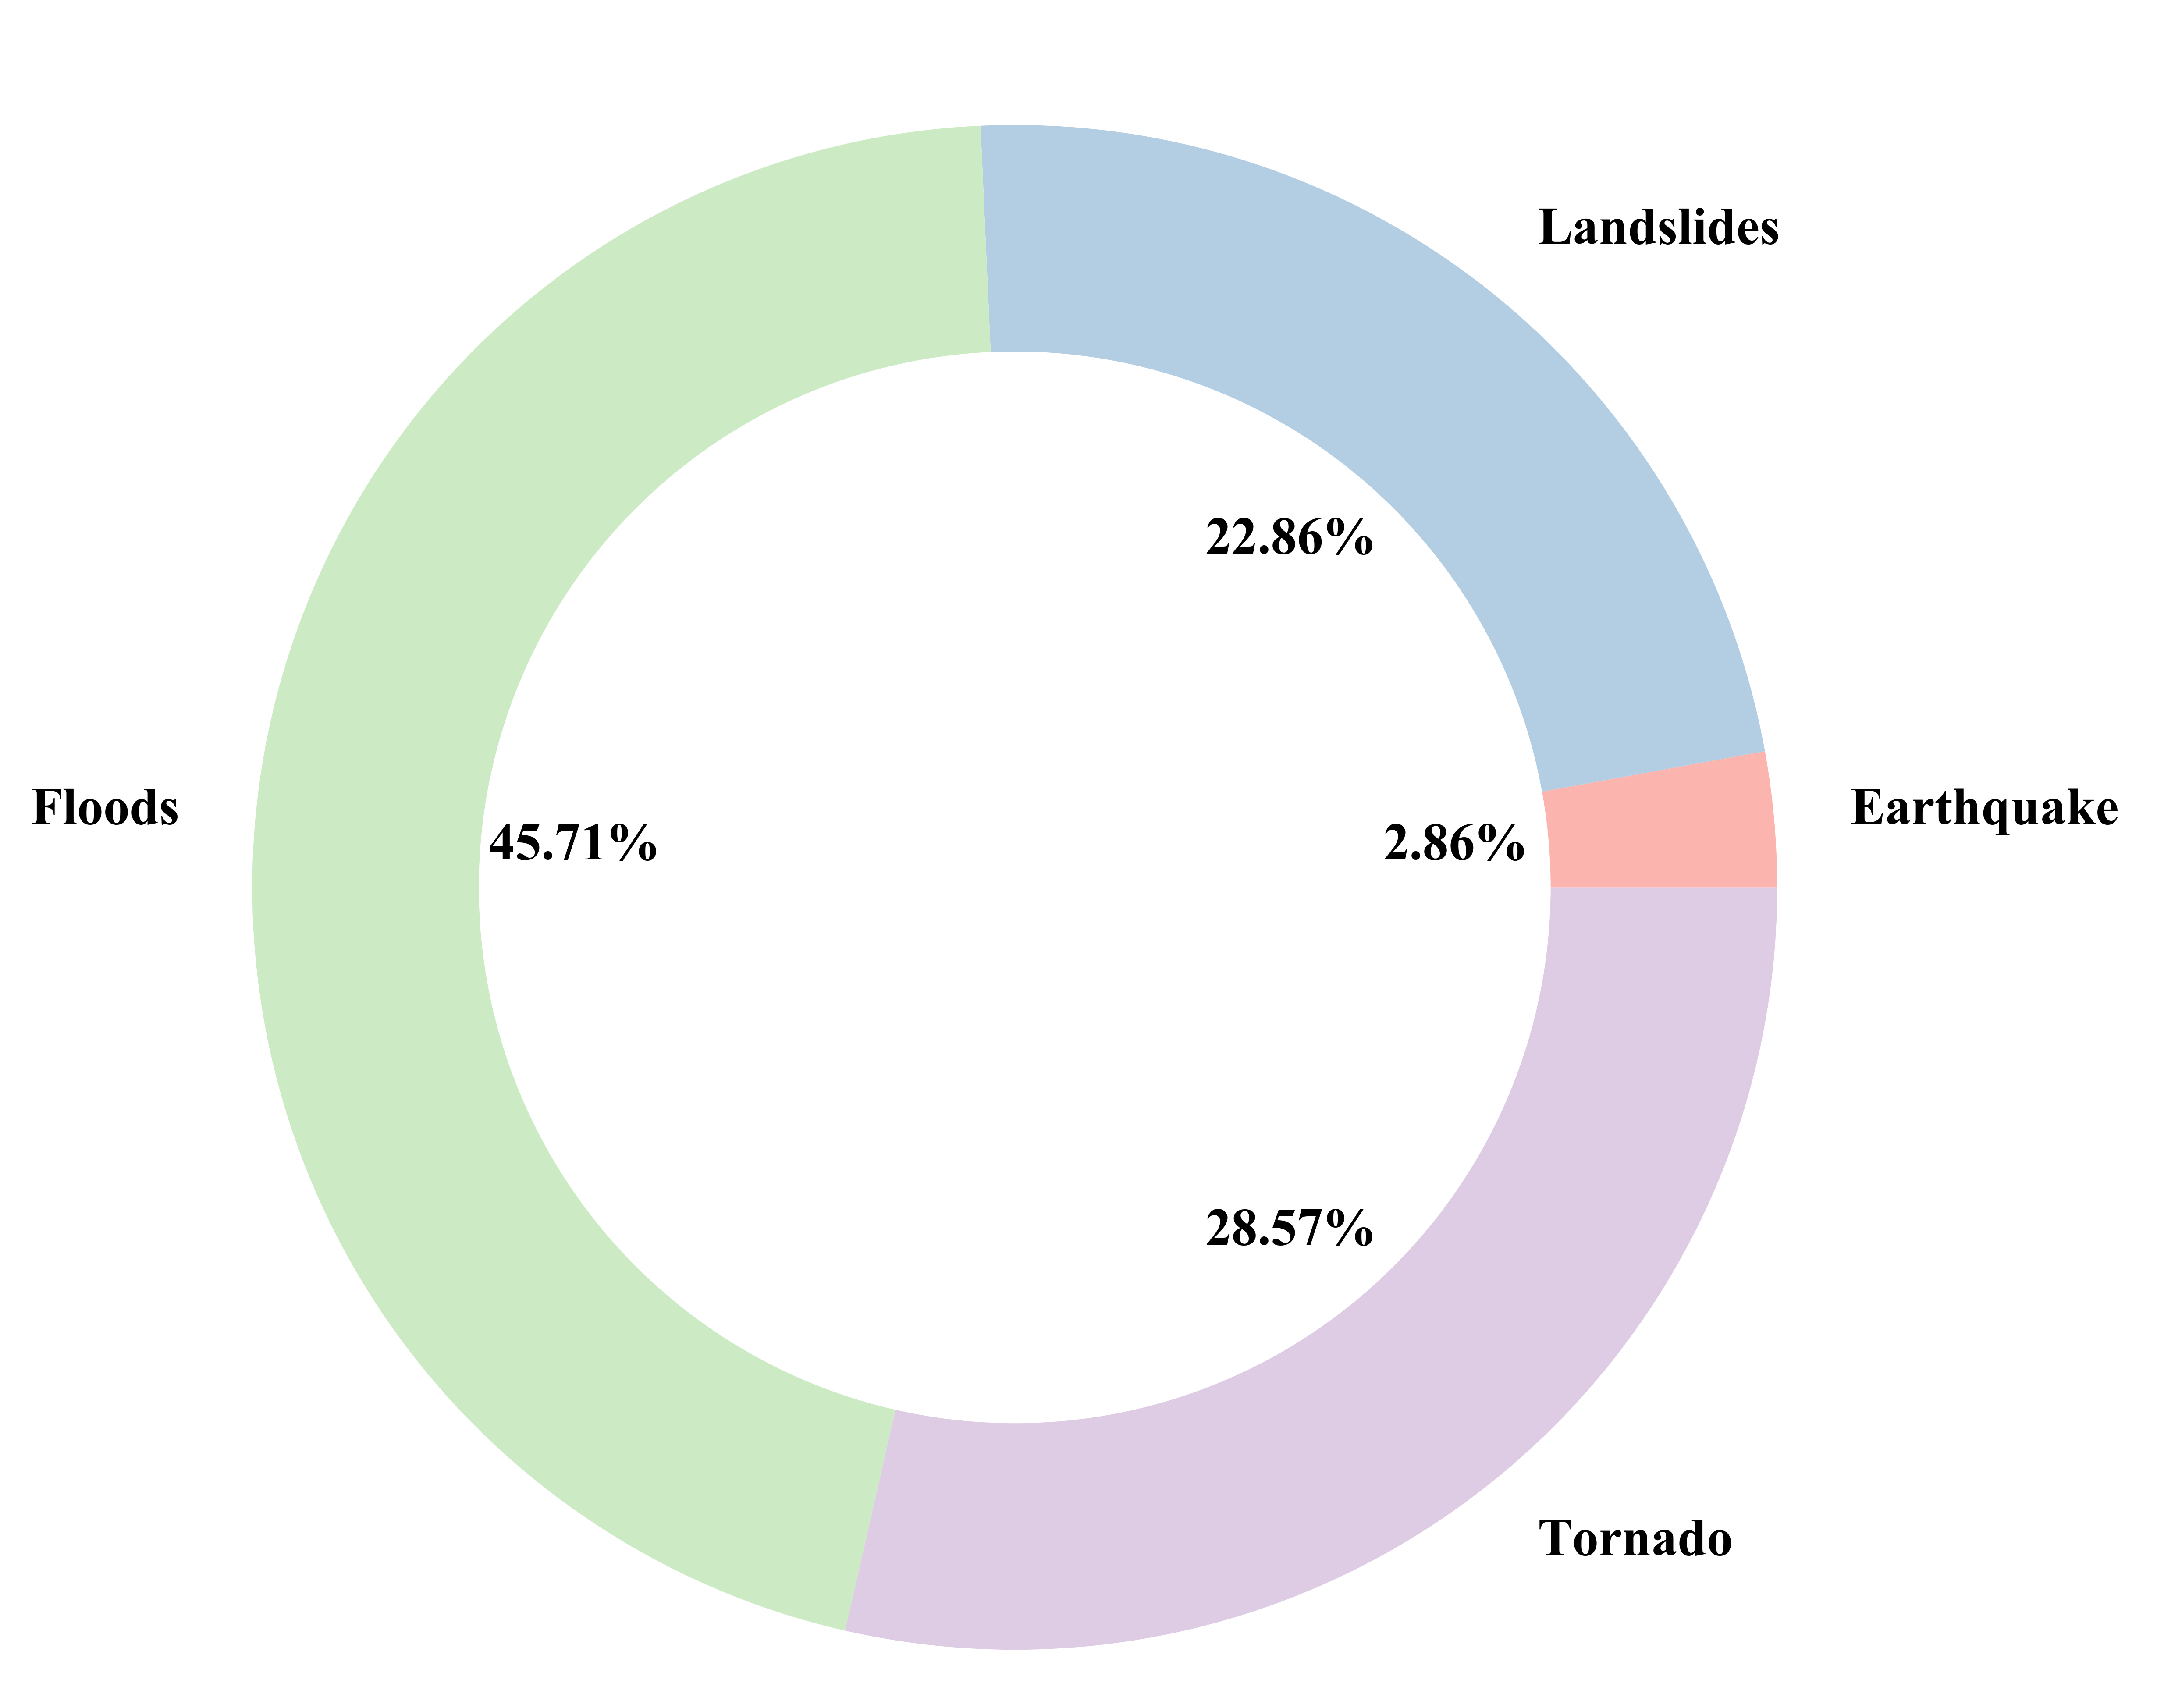
\includegraphics[scale=0.15]{foo.png}
\caption{Natural disasters occurred in Jakarta throughout 2018}
\end{center}
\end{figure}

\section{Motivation}

Based on the problem description above, it will be interesting to understand more of the nature of floods in Jakarta by utilizing the available public data. By using the data, the association between different types of variables can be drawn and an insight about why, when, or where the floods will occur in any given time can be predicted. Such an insight will be beneficial for the government, local authorities, the rescue teams, the medical teams, as well as all of the residents to have strategic measurements against upcoming floods.\\

\noindent
In this project, there are four main topics that will be discussed:
\begin{enumerate}
  \item The possible explanatory variable for the flood occurrence in Jakarta, in particular the rainfall rate, will be investigated. Then, the possible correlation between rainfall rate and the flood trends in Jakarta sub-districts throughout the year 2013 until 2017 will be studied. 
   \item The possible correlation between the rainfall rate with the amount of sub-district and people that will be affected by floods is also going to be studied. Based on possible correlation between these variables, a predictive modeling algorithm will be applied to predict future floods and their potential collateral damage.
   \item Based on the knowledge acquired from point number 1 and point number 2, the districts in Jakarta will be clustered into several segments to find out which districts that have potentially high or low risks of floods should a heavy rainfall pours down the city. 
   \item A variable that might be beneficial to mitigate floods, which is the amount of parks in each district, will be studied. To understand the correlation between the amount of parks and the severity of floods in each district, Pearson correlation method will be used.
\end{enumerate}

\section{Data Sources}
In order to conduct all of the steps in the motivation sections above, data from different sources will be used. 
\begin{enumerate}
\item The data regarding the rainfall rate will be fetched from the BPS website. The website contains public open datasets which are accessible to anybody. However, due to the limitations of the data, the rainfall rate that is going to be considered will be the rate in the span of 2013 until 2017.
\item The data regarding the amount of sub-districts as well as the number of people who are affected by floods will be fetched from Satu Data Indonesia, which is a website contains of several open datasets from the Indonesian government regarding national issues. Due to data limitations, the data that will be investigated is also going to be in the span of 2013-2017.
\item In order to get the name of all of the districts in Jakarta, the web-scraping approach from Wikipedia page will be applied.
\item To obtain the complete latitude and longitude coordinates for all of the districts in Jakarta, geopy library will be used.
\item In order to obtain the data regarding the amount of parks in any given districts, the Foursquare API will be used. Then, additional filtering of the data obtained from Foursquare API will be conducted if necessary. 
\end{enumerate}

\section{Data Features}
In this section, the features of the data sources that has been explained in the previous section will be explained.
\begin{enumerate}
\item \textbf{Data from the BPS:} There is one csv file from BPS website that contains the rainfall rate in any given month throughout the year 2009 until 2017. However in order to match the available data regarding the flood occurrences that will be explained in point number two, only the rainfall rate in the span of 2013 until 2017 will be considered.
\item  \textbf{Data from Satu Data Indonesia:} there are two different types of datasets that will be fetched from this website:

\begin{itemize}
\item Five csv files (2013 until 2017) in which each file contains an information about the flood occurrences in a given year (annual floods recapitulation).
\item More than 30 csv files that will be combined into a data frame in which each of the csv file contains an information about flood occurrences in a month from 2013 until 2016. The features that can be obtained from each file including the number of sub-districts affected by flood, the number of people affected by floods, days needed for each sub-district to recover from flood, and the number of people who are forced to relocate from their own house because of floods in any given month.
\end{itemize}
\item \textbf{Data from Wikipedia page:} there will be five different pages from Wikipedia that will be used to obtain the complete districts name of Jakarta. The url of each of the website is going to be listed in the Reference section.
\item \textbf{Data from Foursquare API:} with Foursquare API, a specific category of the place of interest can be defined in advance. In this project, a specific category, which is parks, will be used to obtain the list of the parks located in each district of Jakarta.
\end{enumerate}
\chapter{Understanding Rainfall Rate and Flood Occurrences}

In this chapter, one of the potential explanatory variable for the flood occurrences in Jakarta, which is the rainfall rate, will be investigated. \\

\section{Rainfall Rate Throughout the Year 2013 Until 2017}

The rainfall rate data in a csv file format is obtained from the BPS website and this data is open for anybody to use it. The csv file contains monthly rainfall rate from the year of 2009 until 2017. However, to accommodate the available flood occurrences data, the rainfall rate that will be considered are the rate in the span of 2013 until 2017. Figure \ref{fig=rainfall.png} shows the trends of the rainfall rate in Jakarta throughout 2013 until 2017.\\

\begin{figure}
\begin{center}
\graphicspath{ {./Pict/} }
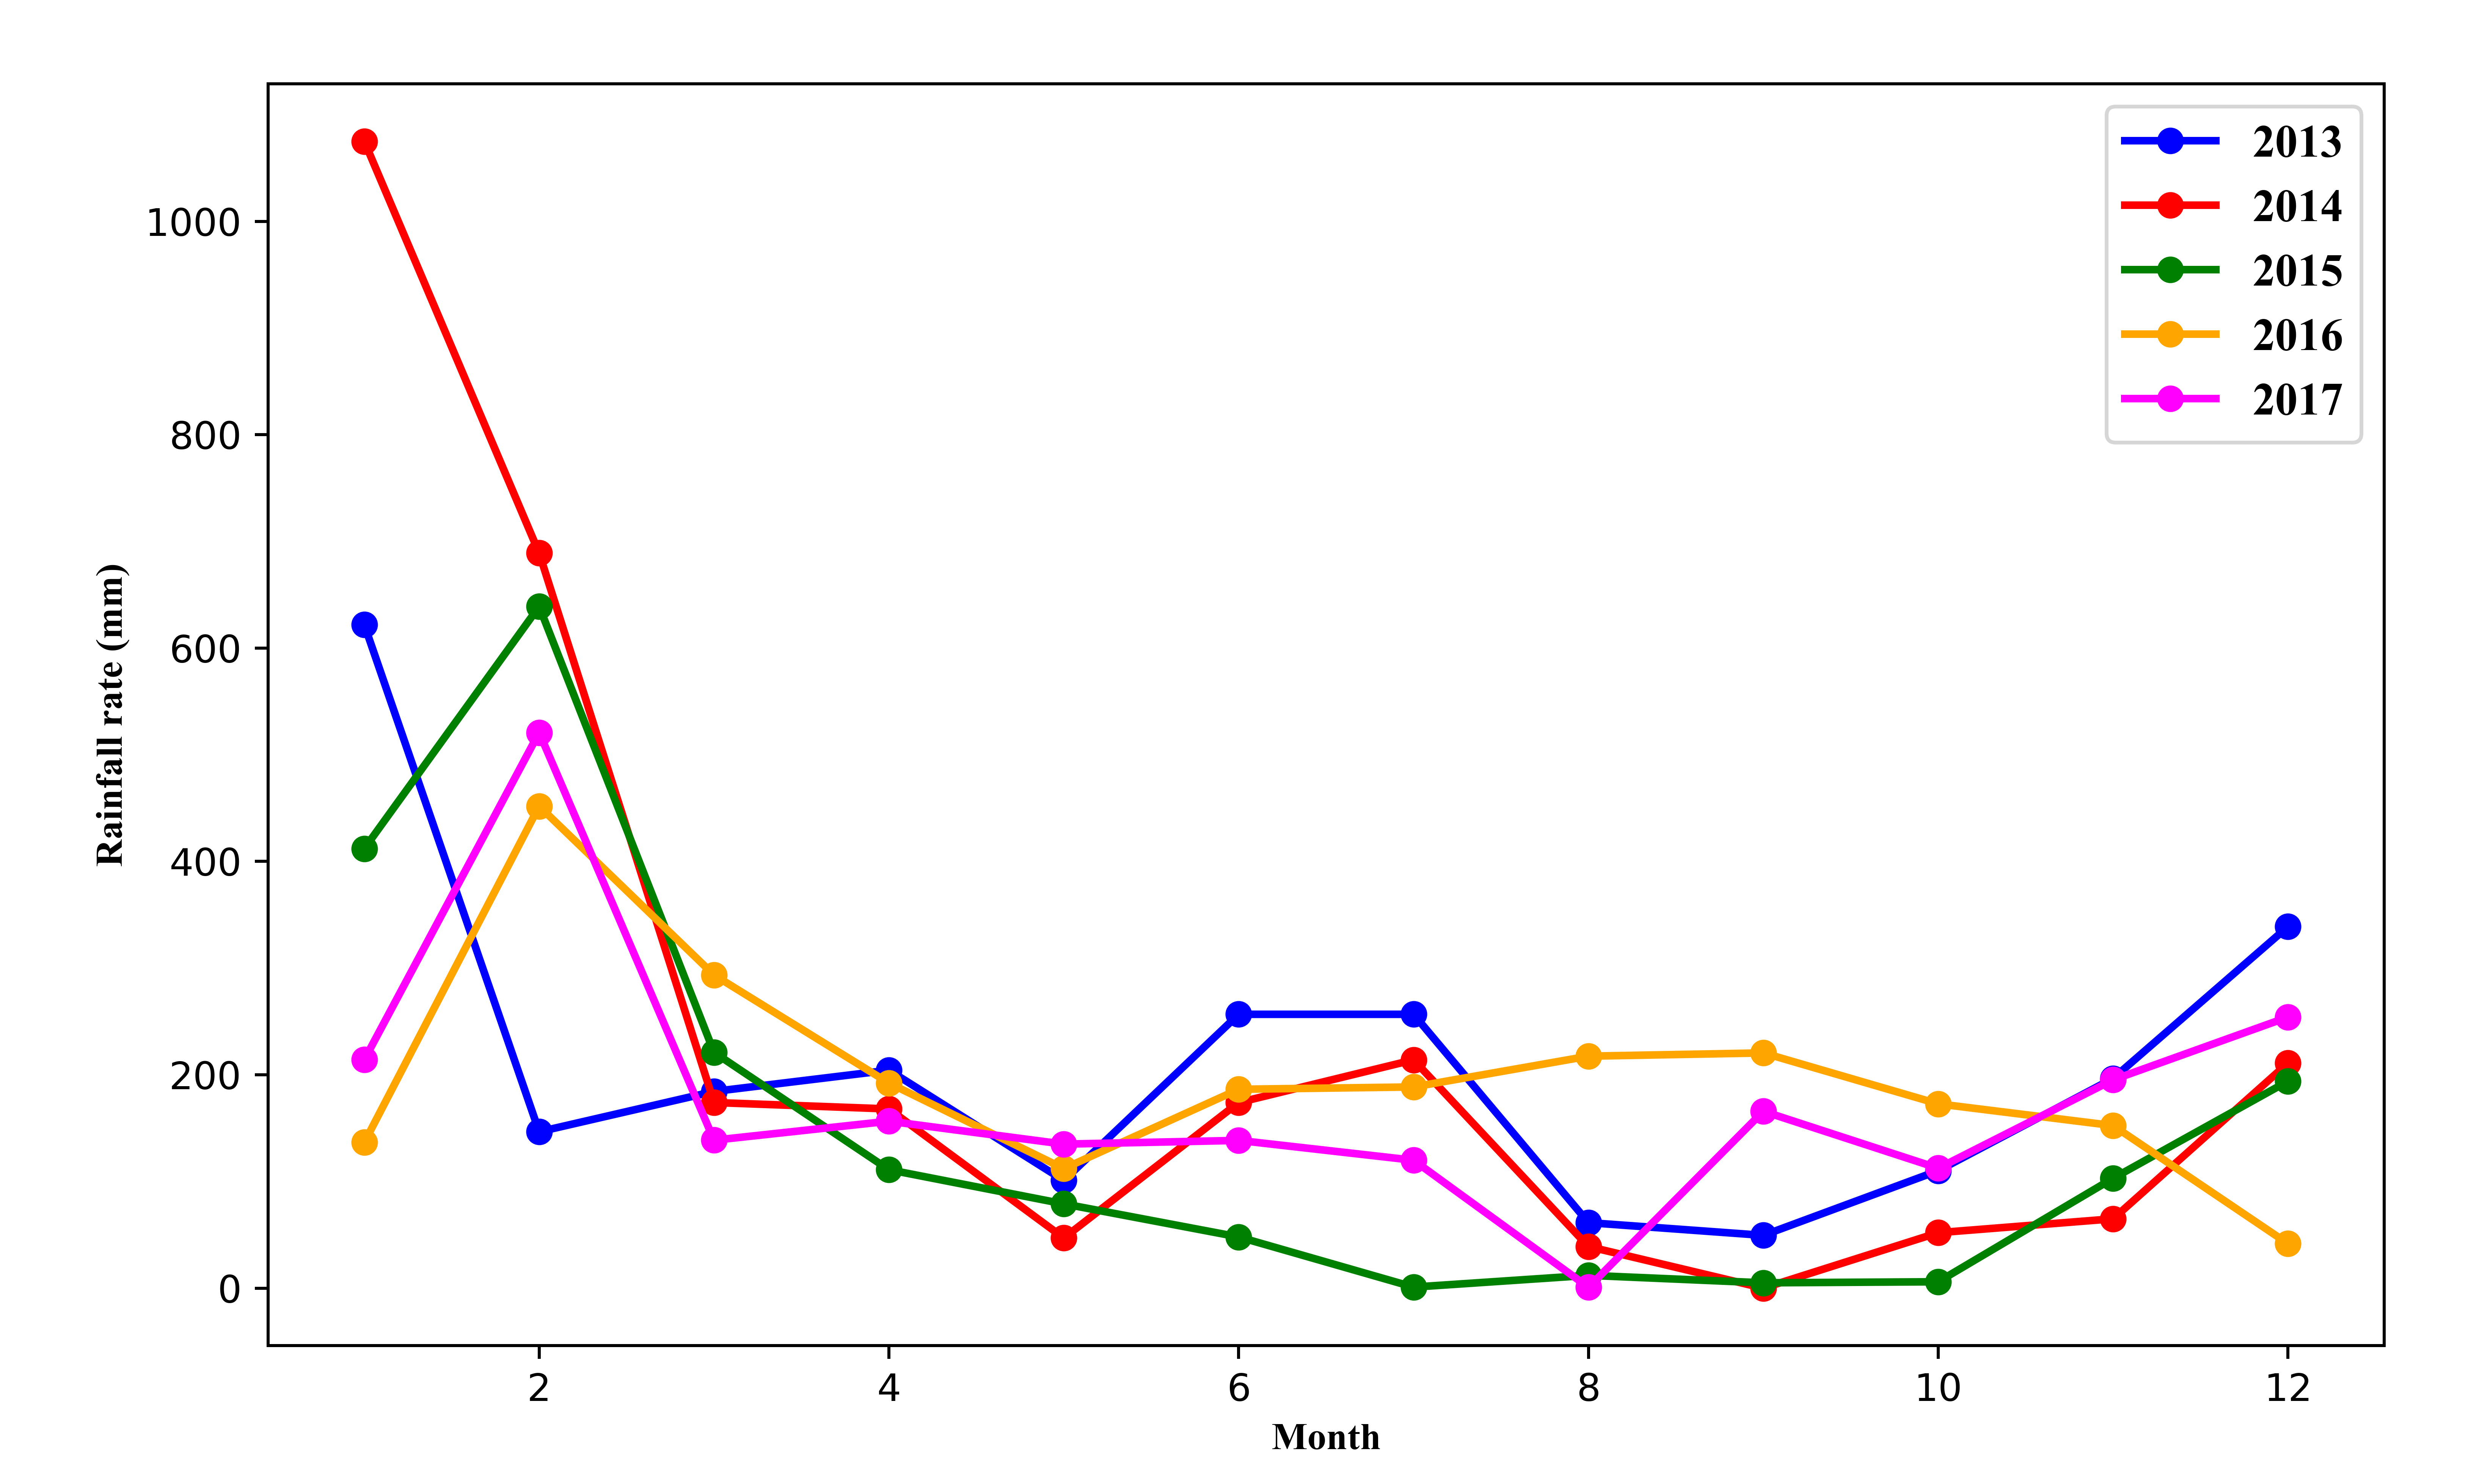
\includegraphics[scale=0.15]{rainfall.png}
\caption{Rainfall rate in Jakarta throughout 2013-2017}\label{fig=rainfall.png}
\end{center}
\end{figure}

\noindent
From Figure \ref{fig=rainfall.png}, it can be seen that there are certain patterns regarding the rainfall rate in any given year. In general, the rainfall rate reach its highest in January and February. Then, from March and the following month the rate is gradually dipping until it  reaches its lowest point between the month of August until October before it starts to increase again from November and so on. \\

\noindent
However, before drawing any conclusion from Figure \ref{fig=rainfall.png}, the trends regarding the flood occurrences in Jakarta throughout 2013 until 2017 needs to be investigated first. This is necessary to check whether there might be a correlation between flood occurrences and rainfall rate.

\section{Flood Occurrences Throughout the Year 2013 Until 2017}

Before visualizing the trend regarding the flood occurrence in Jakarta, first a variable to quantify the occurrence of floods needs to be defined. In order to quantify the flood occurrence, the number of sub-districts that have been affected by floods in any given month throughout 2013 until 2017 is investigated. Figure \ref{fig=flood.png} shows the amount of sub-districts in Jakarta that have been affected by floods from 2013 until 2017.\\

\begin{figure}
\begin{center}
\graphicspath{ {./Pict/} }
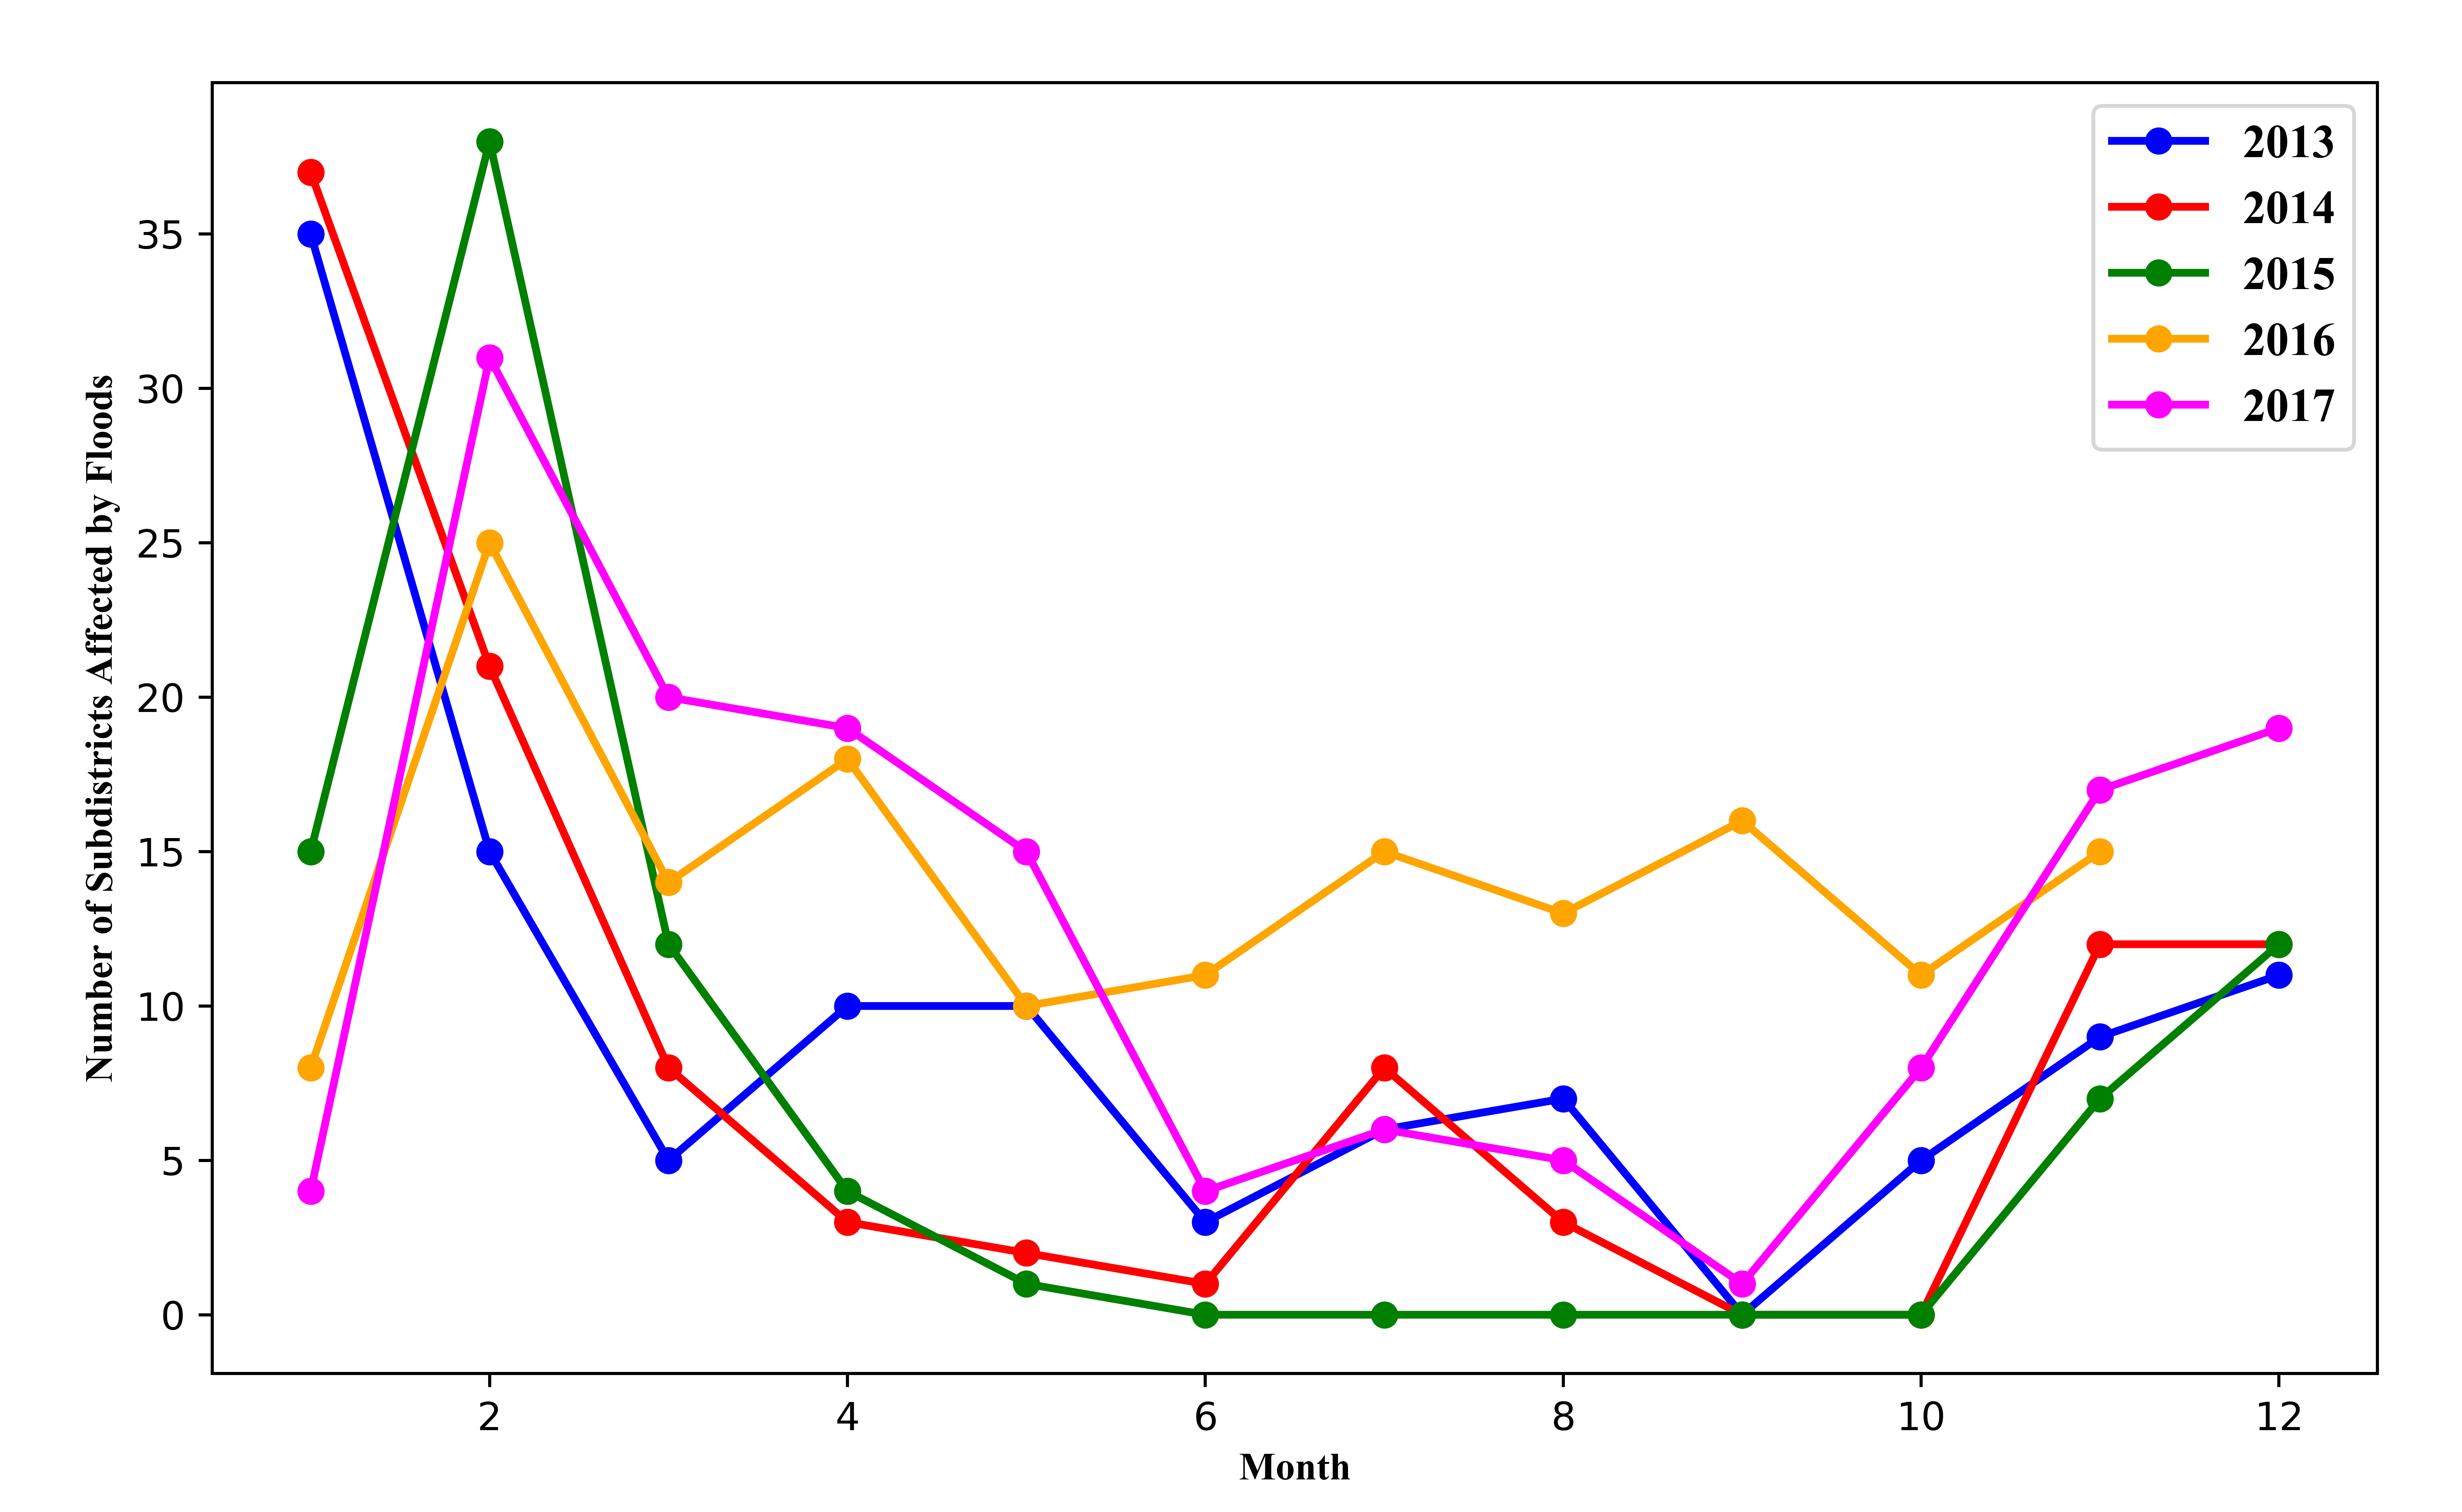
\includegraphics[scale=0.15]{flood.png}
\caption{Flood occurrences in Jakarta throughout 2013-2017}\label{fig=flood.png}
\end{center}
\end{figure}

\noindent
From Figure \ref{fig=flood.png}, it can be concluded that there are similar patterns of flood occurrences and rainfall rate. The flood case in Jakarta reach its highest during January and February, in which at least five districts affected by floods. Then, starting from March and the following month the flood occurrence is decreasing until reaches its lowest starting in June until October before it starts to increase again on November and so on.\\

\noindent
Because of the similarity of patterns between rainfall rate and flood occurrences, hence it can be concluded that there are positive correlation between one another. However, the direct correlation between these two variables will be discussed in more detail in the next chapter. \\

\noindent
From the Figure \ref{fig=rainfall.png} and Figure  \ref{fig=flood.png}, a suggestion can be made to the authorities and the government regarding the best period of time in a year to prepare some mitigation measurements. Since the flood occurrences and rainfall reach their lowest in around May until October, then it can be suggested that between the month of May until October are the best period of time to do some precautionary and mitigation measurements of the floods.\\



\chapter{Predicting Future Floods and their Potential Collateral Damage}

In this chapter, the association between rainfall rate and the flood occurrences will be discussed in a more detail. In order to do this, the rainfall rate will be compared with two different variables which represent how severe the flood occurrence is: the amount of sub-districts affected by floods and the number of people who are affected by floods.

\section{Rainfall Rate and the Sub-districts Affected by Floods}

From the previous chapter, it can be concluded that there is a positive correlation between rainfall rate and the sub-districts that are affected by floods. In Figure \ref{fig=corrrainsub.png}, the data points regarding the relationship between the rainfall rate and the amount of sub-districts that are affected by floods in any given rate is shown.\\

\begin{figure}
\begin{center}
\graphicspath{ {./Pict/} }
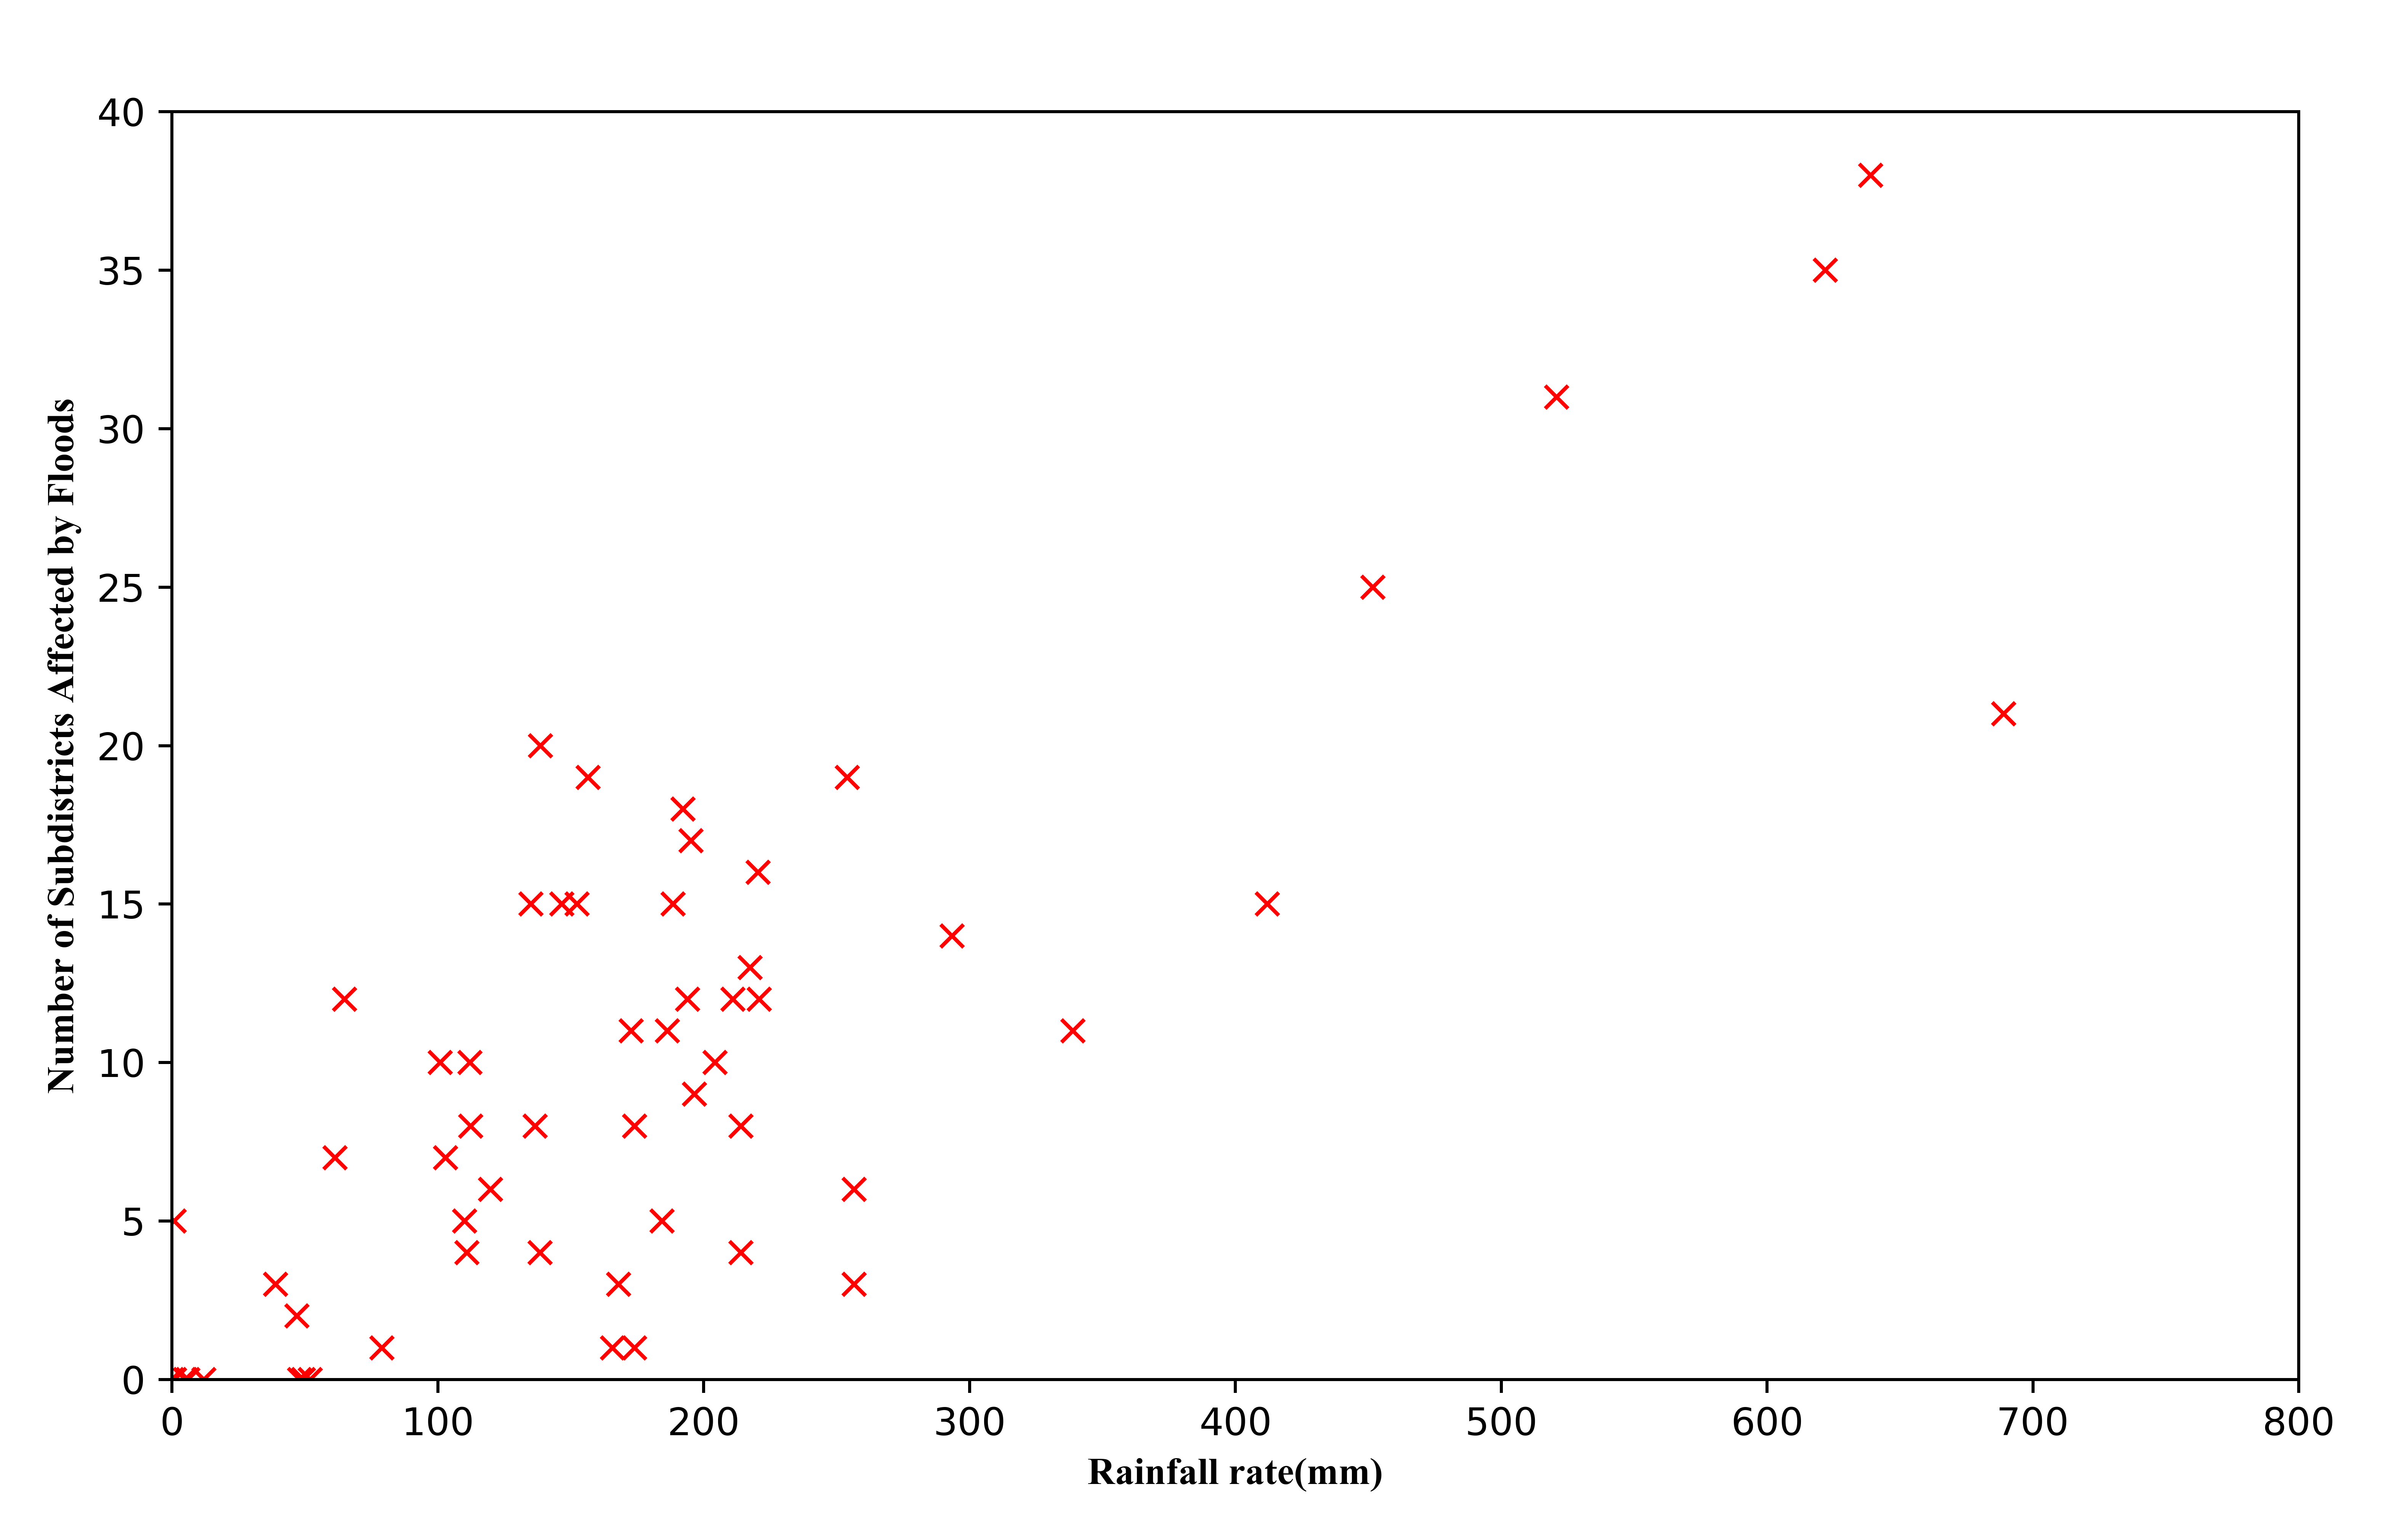
\includegraphics[scale=0.15]{corrrainsub.png}
\caption{Data points of rainfall rate and the sub-districts affected by floods}\label{fig=corrrainsub.png}
\end{center}
\end{figure}

\noindent
From Figure \ref{fig=corrrainsub.png}, it can be clearly seen that there is indeed a positive correlation between rainfall rate and the number of sub-district affected by floods. Also, by looking at the data points, a predictive modeling algorithm can be built. A linear regression model will be the appropriate modeling technique since the variance of the data points looks similar. Figure \ref{fig=corrrainsubreg.png} shows the linear regression model for this particular problem.\\

\begin{figure}
\begin{center}
\graphicspath{ {./Pict/} }
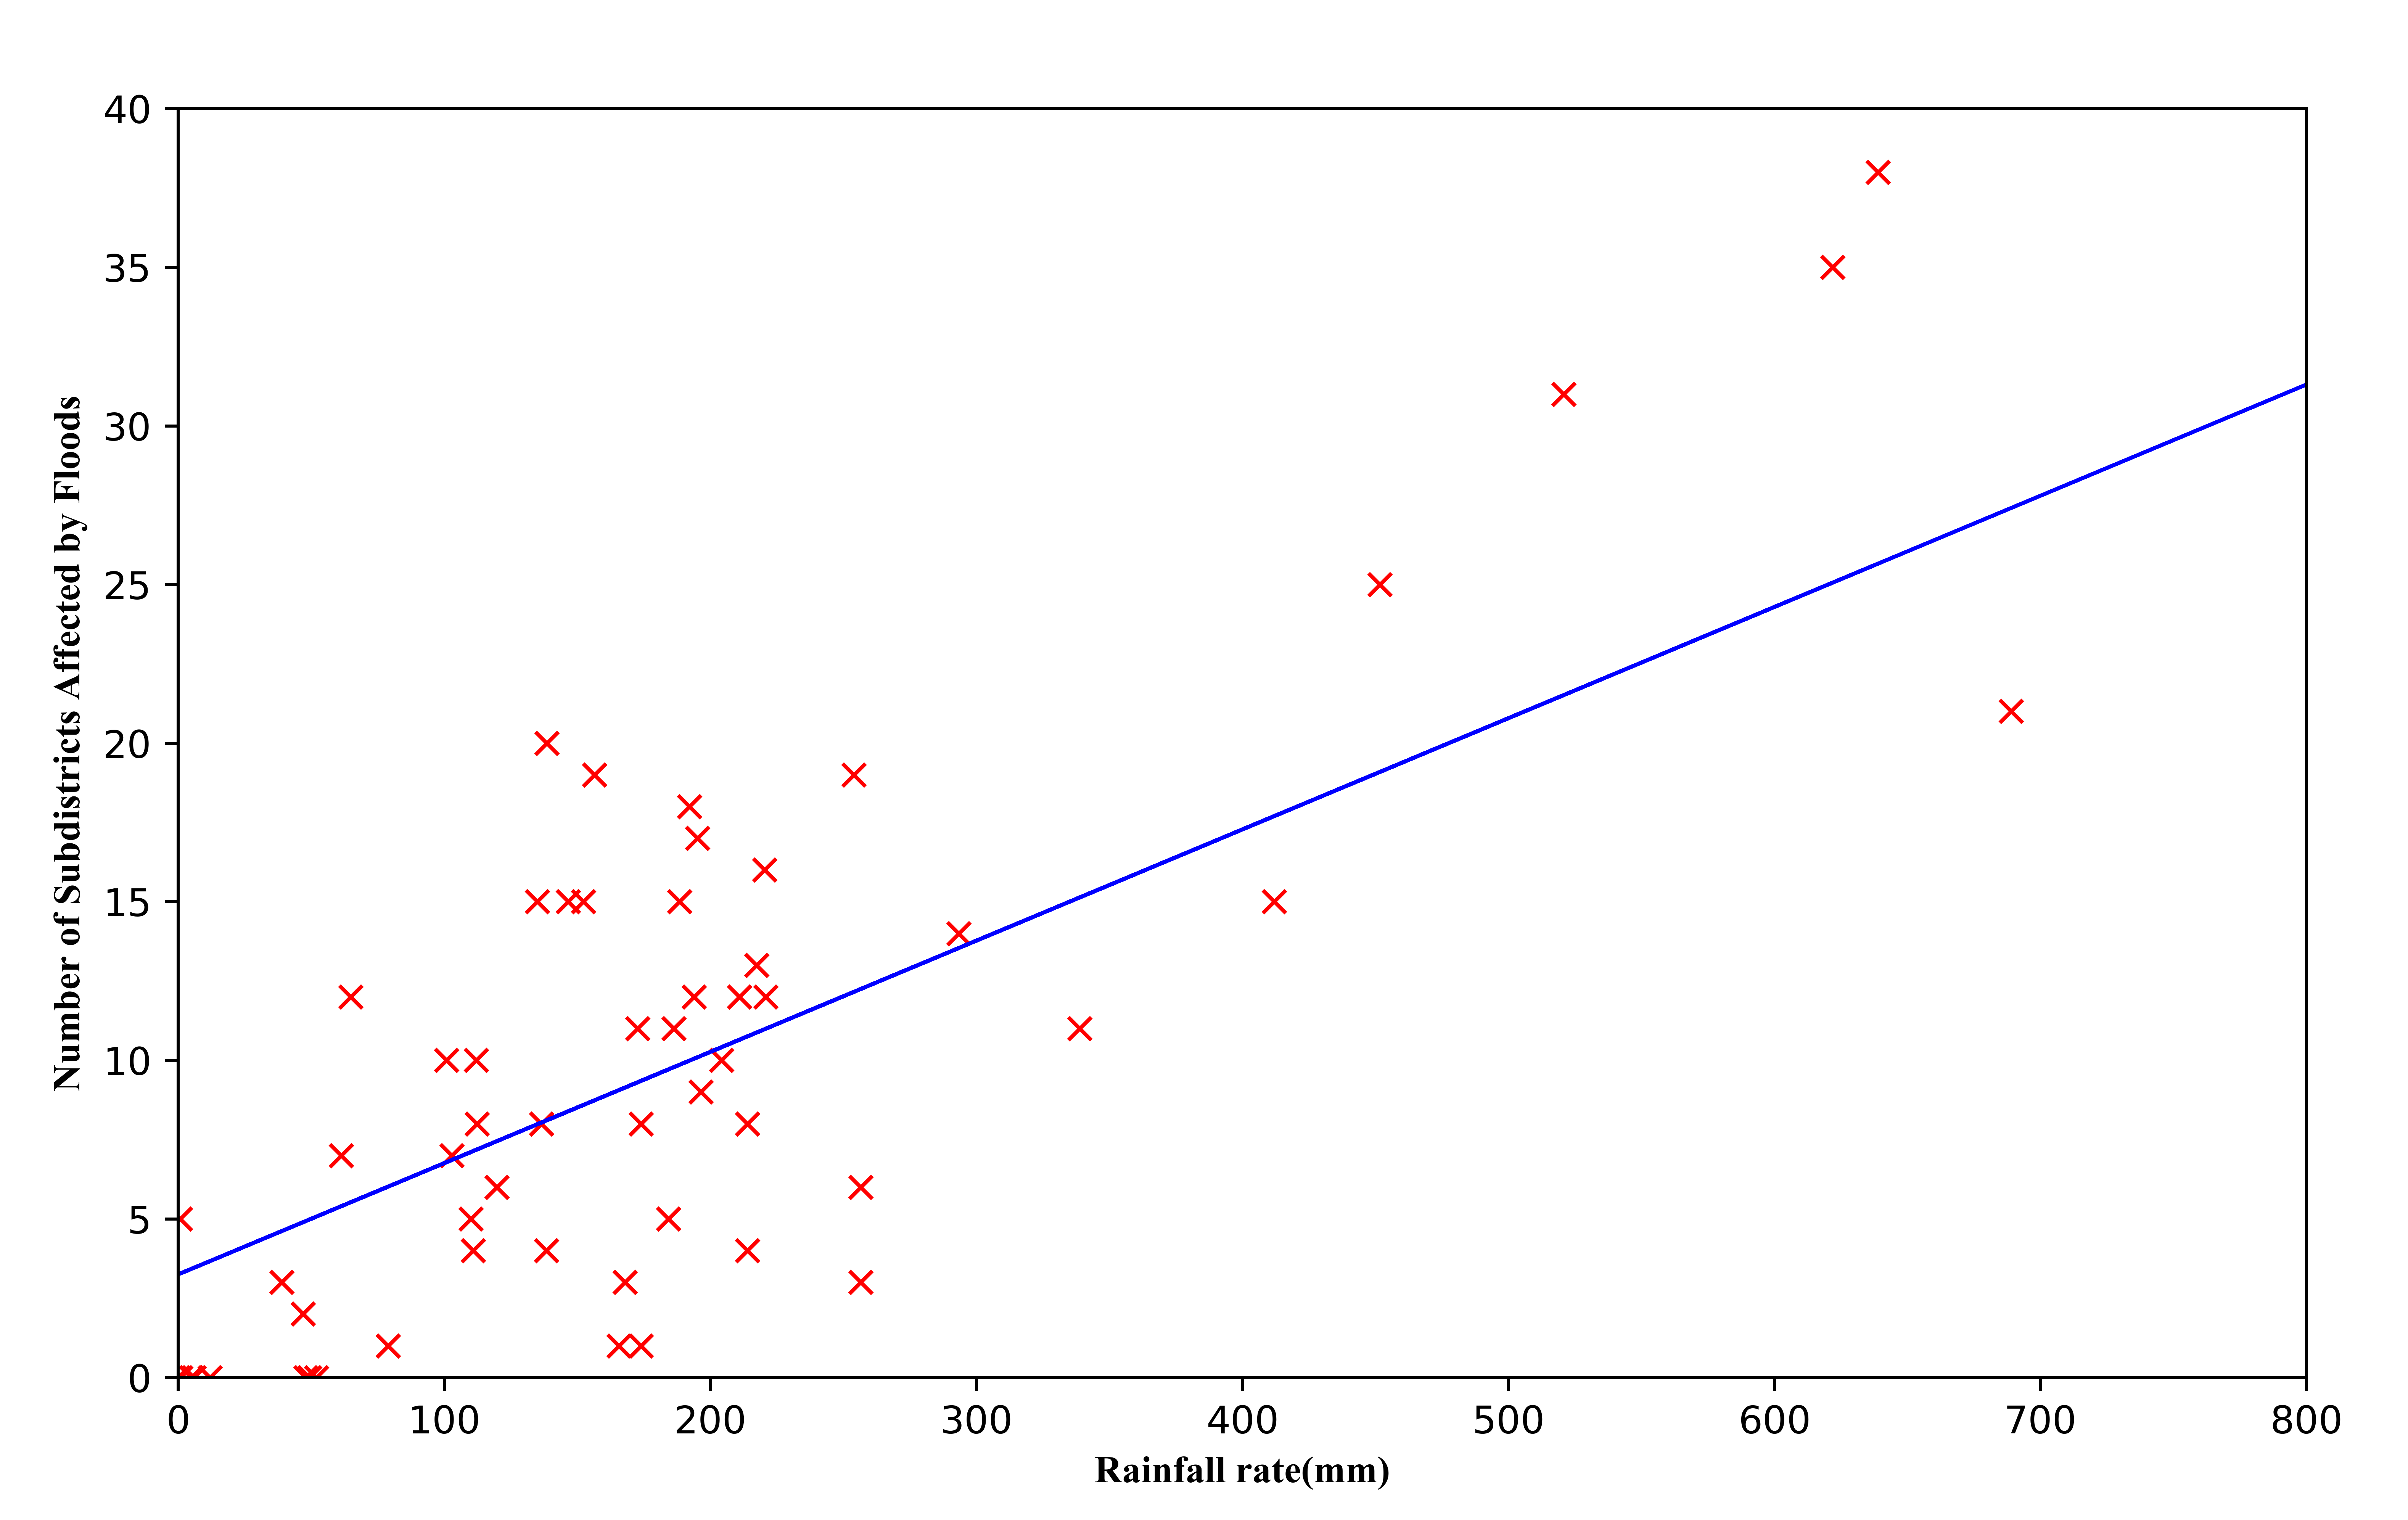
\includegraphics[scale=0.15]{corrrainsubreg.png}
\caption{Linear regression model to estimate the sub-districts affected by floods in any given rainfall rate}\label{fig=corrrainsubreg.png}
\end{center}
\end{figure}

\noindent
With the linear model, now the amount of sub-districts that will be affected by floods in any given rainfall rate can be estimated and prepared. The ability to predict the amount of sub-districts that will be affected by floods would be particularly important for the authorities to conduct some flood mitigation measurements in certain sub-districts.

\section{Rainfall Rate and the People Affected by Floods}
By now, it can be concluded that the amount of sub-districts that will be affected by floods can be estimated using a linear regression model. But how about the number of people who are affected by floods? To answer the question, similar steps as before will be conducted.\\

\noindent
Generally, one can assume that if the amount of sub-district affected by floods has a more or less linear correlation with the rainfall rate, then the same correlation applies for the number of people who are affected by floods. But does it? Figure \ref{fig=corrrainpeop.png} shows the correlation between two variables.\\

\begin{figure}
\begin{center}
\graphicspath{ {./Pict/} }
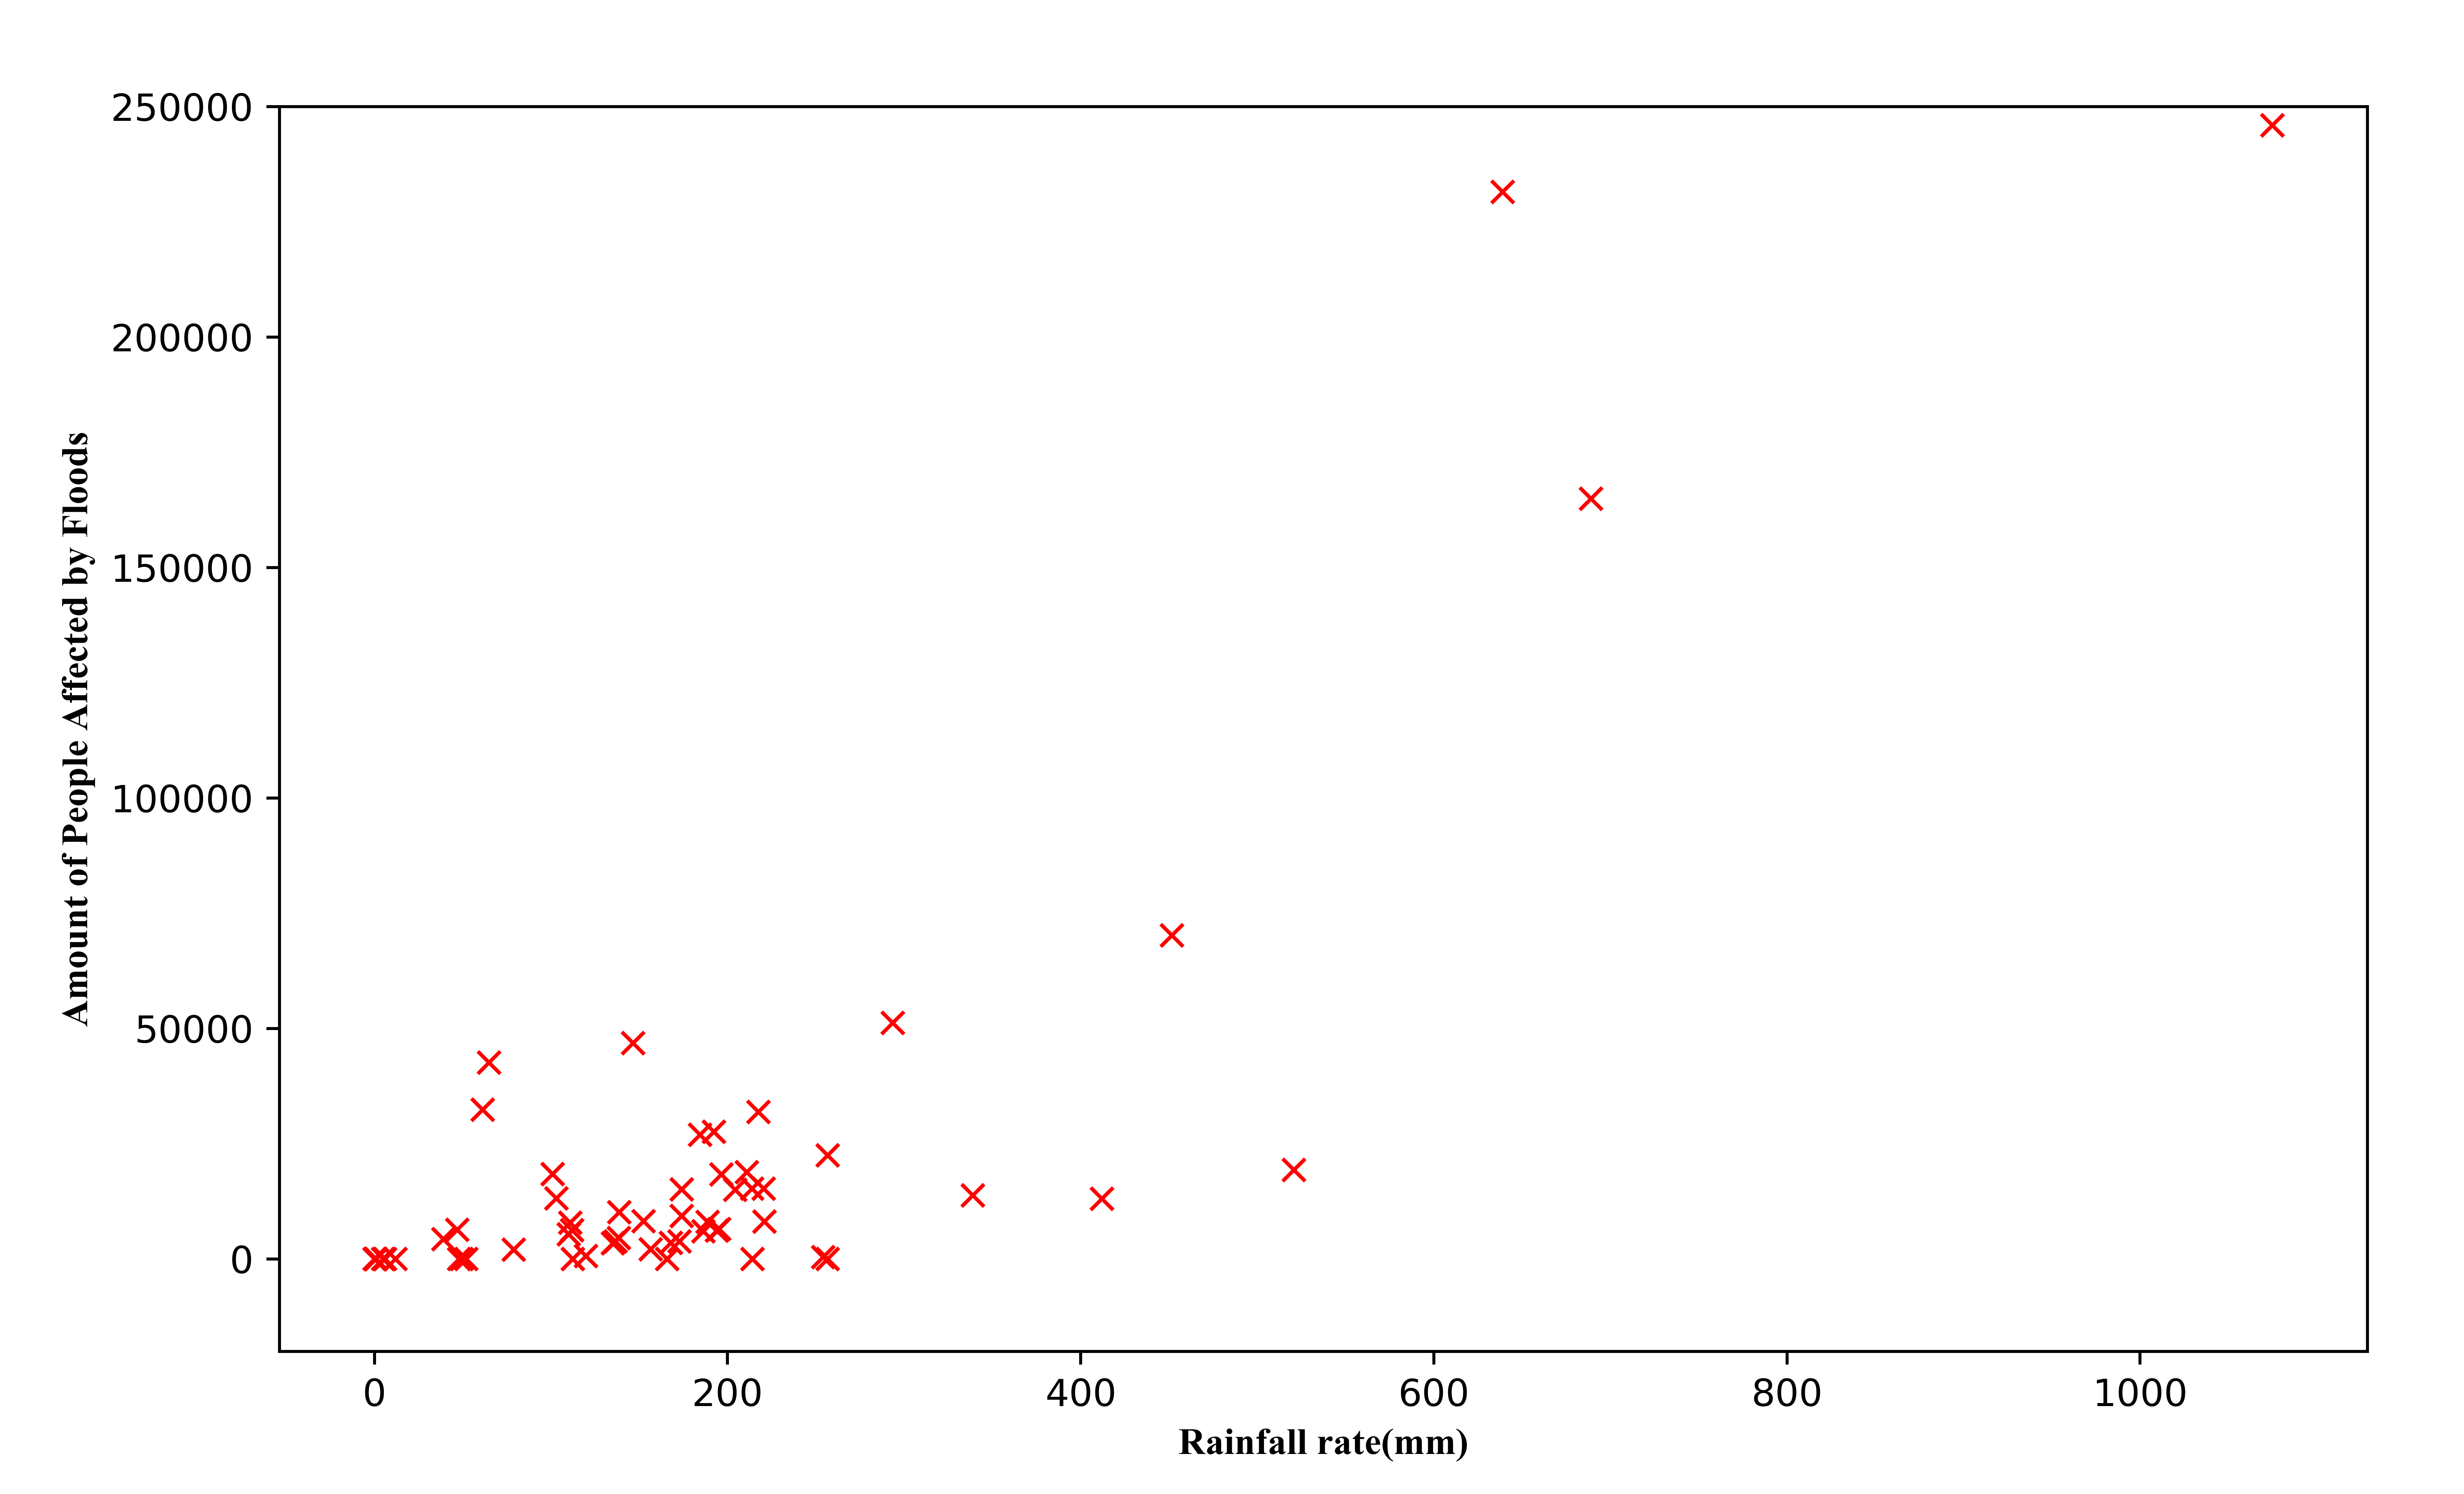
\includegraphics[scale=0.15]{corrrainpeop.png}
\caption{Data points of rainfall rate and the amount of people who will be affected by floods}\label{fig=corrrainpeop.png}
\end{center}
\end{figure}

\noindent
From Figure \ref{fig=corrrainpeop.png}, it can be concluded that rainfall rate also has a positive correlation with the amount of people who are affected by floods. However, by just looking at the data points, a linear model would not be an optimal model to predict the amount of people who are affected by floods because of the linearity characteristics wouldn't be able to catch the trend in the data points. Hence, a polynomial regression model will be more suitable for this particular problem.\\

\noindent
Before a polynomial regression model is applied, it is important to check which order that might be suitable for the problem. As an evaluation metric, R-squared or coefficient of determination is used. Figure \ref{fig=rsquare.png} shows how the R-squared score looks like when a polynomial regression model with variety of orders is applied within the test data of the data points in Figure \ref{fig=corrrainpeop.png}. As shown already, as the order of the polynomial model is higher than 4, the R-squared score is gradually decreasing. This phenomenon is a sign of overfitting since the model is trying to fit-in the data points which in turns give a high error and low number of R-squared.\\

\begin{figure}
\begin{center}
\graphicspath{ {./Pict/} }
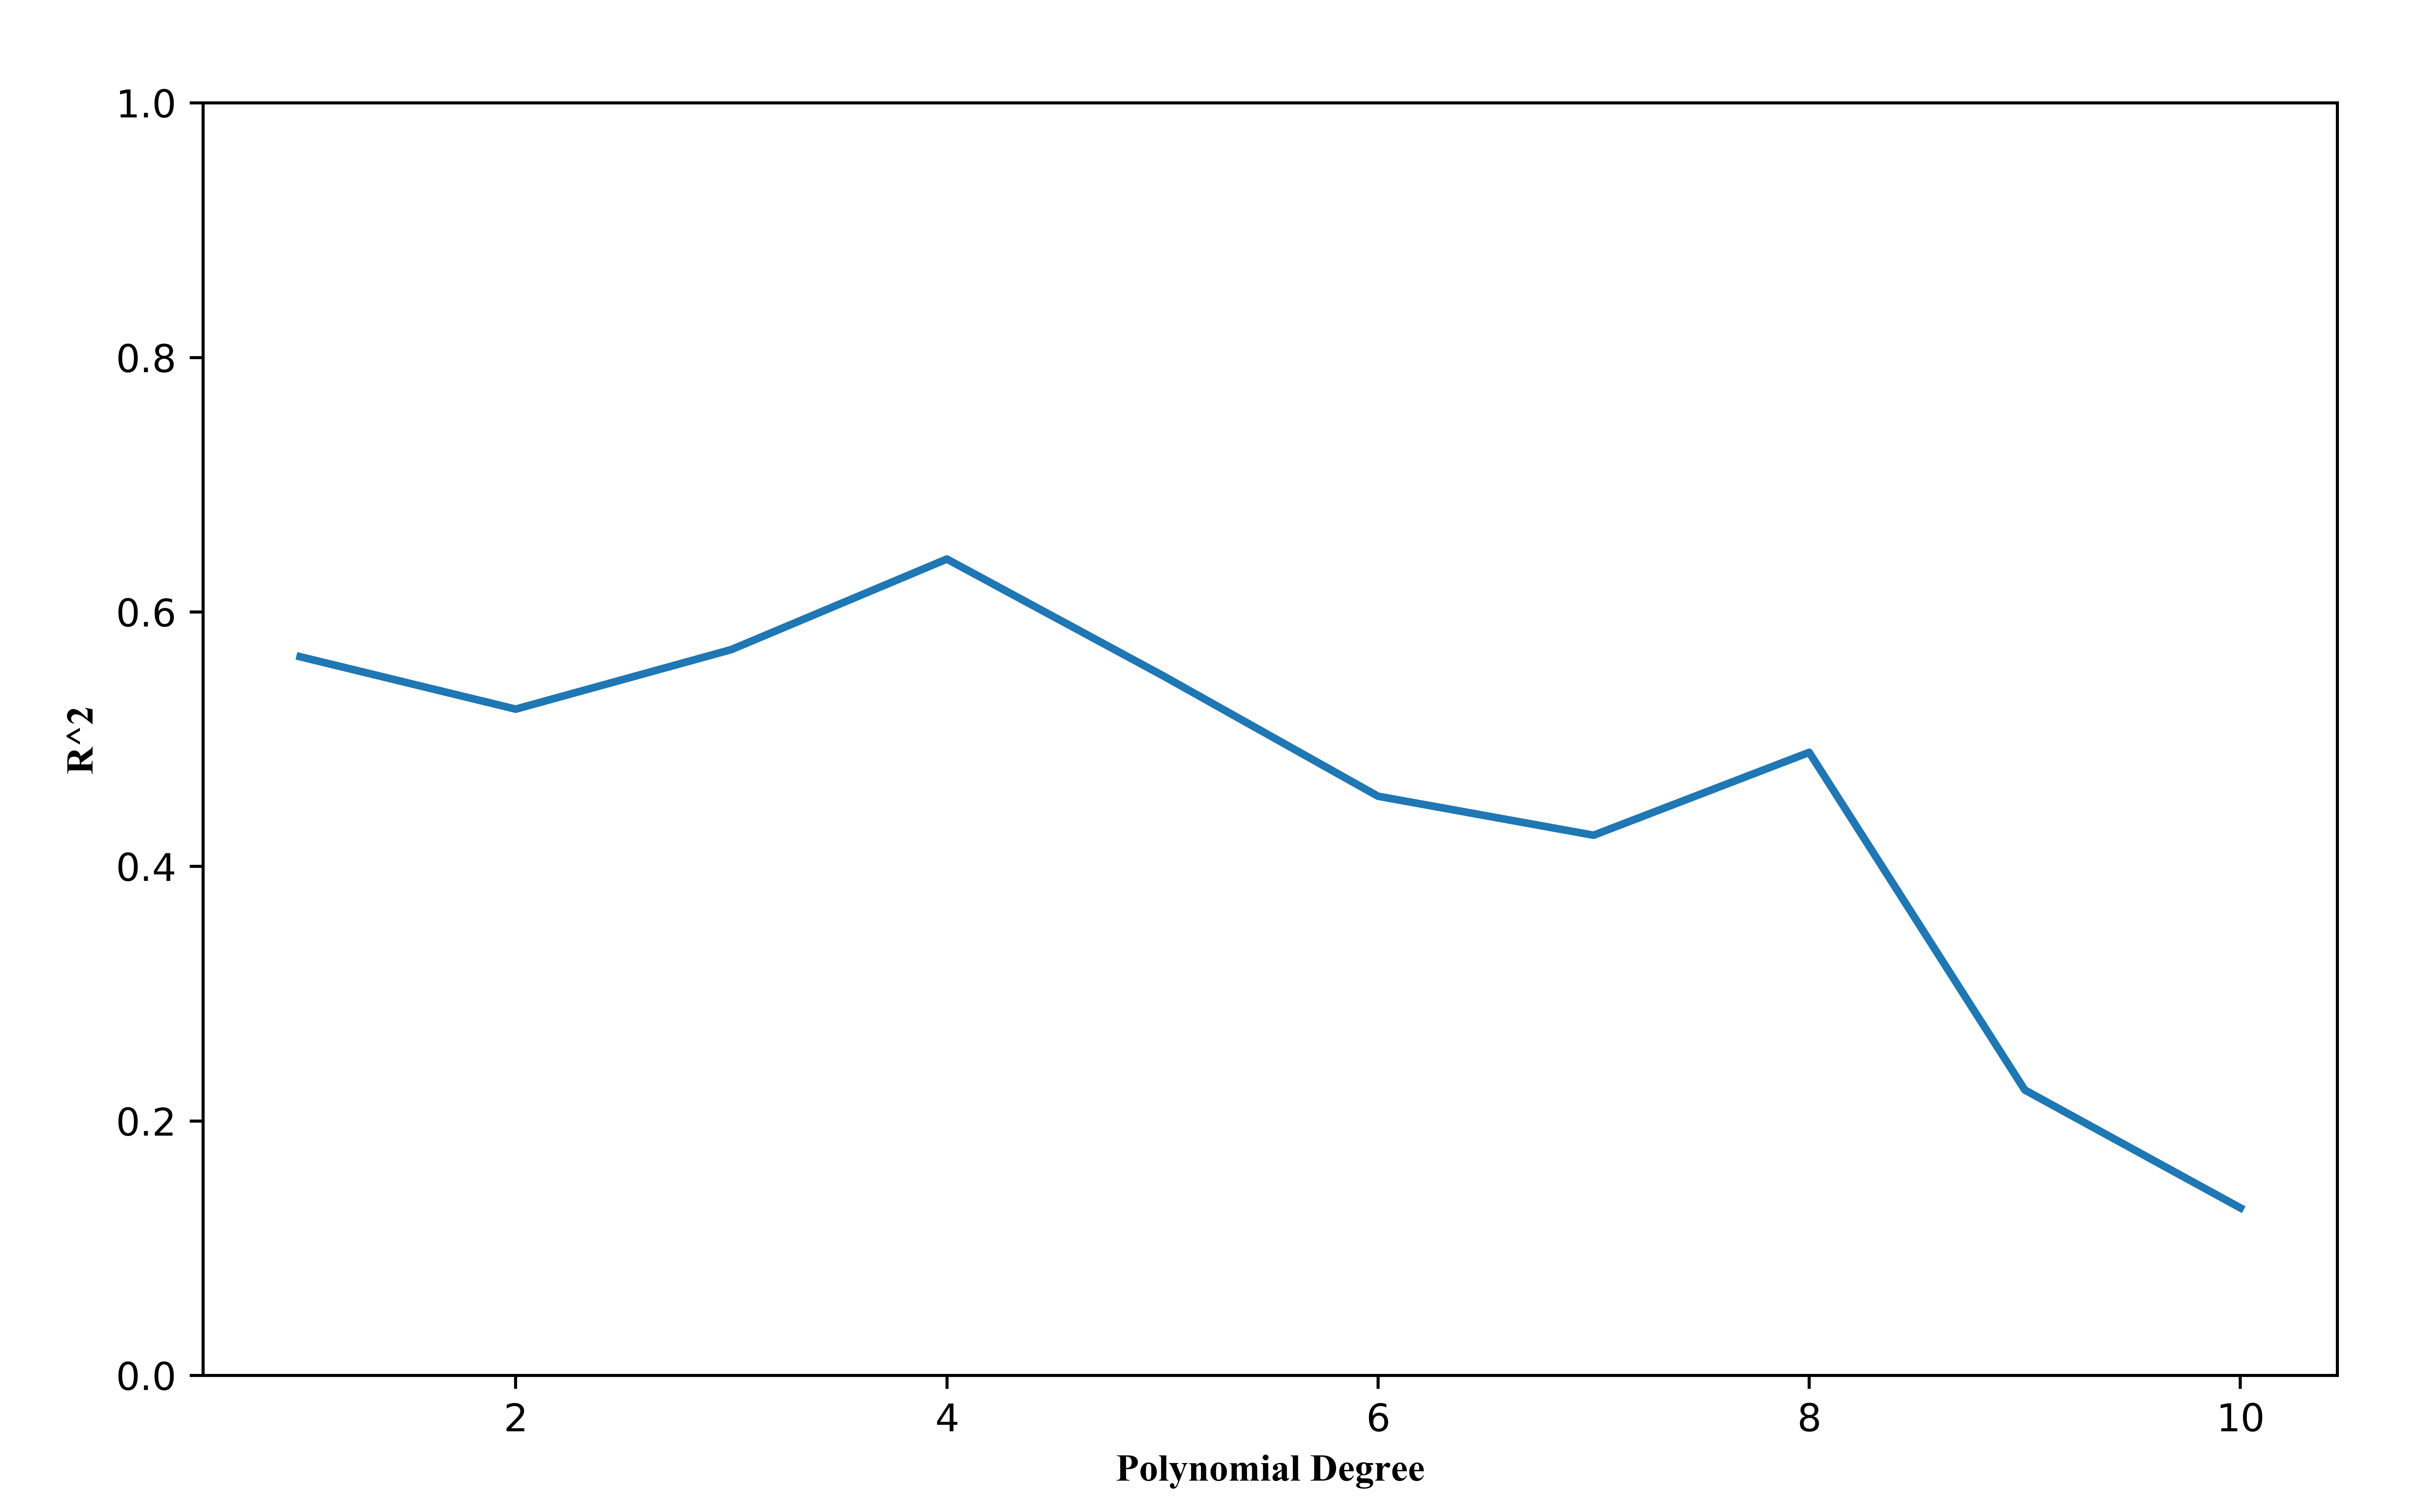
\includegraphics[scale=0.15]{rsquare.png}
\caption{R-squared score of polynomial models with variety of orders when predicting the test data}\label{fig=rsquare.png}
\end{center}
\end{figure}

\noindent 
Based on the Figure \ref{fig=rsquare.png}, polynomial model with order in between two until four will be good candidates. In order to find which order will fits and best to generalize the data points in this particular problem, several graphs are created, as shown in Figure \ref{fig=pol24.png} and Figure \ref{fig=corrrainpeopreg.png}.\\

\begin{figure}
\begin{center}
\graphicspath{ {./Pict/} }
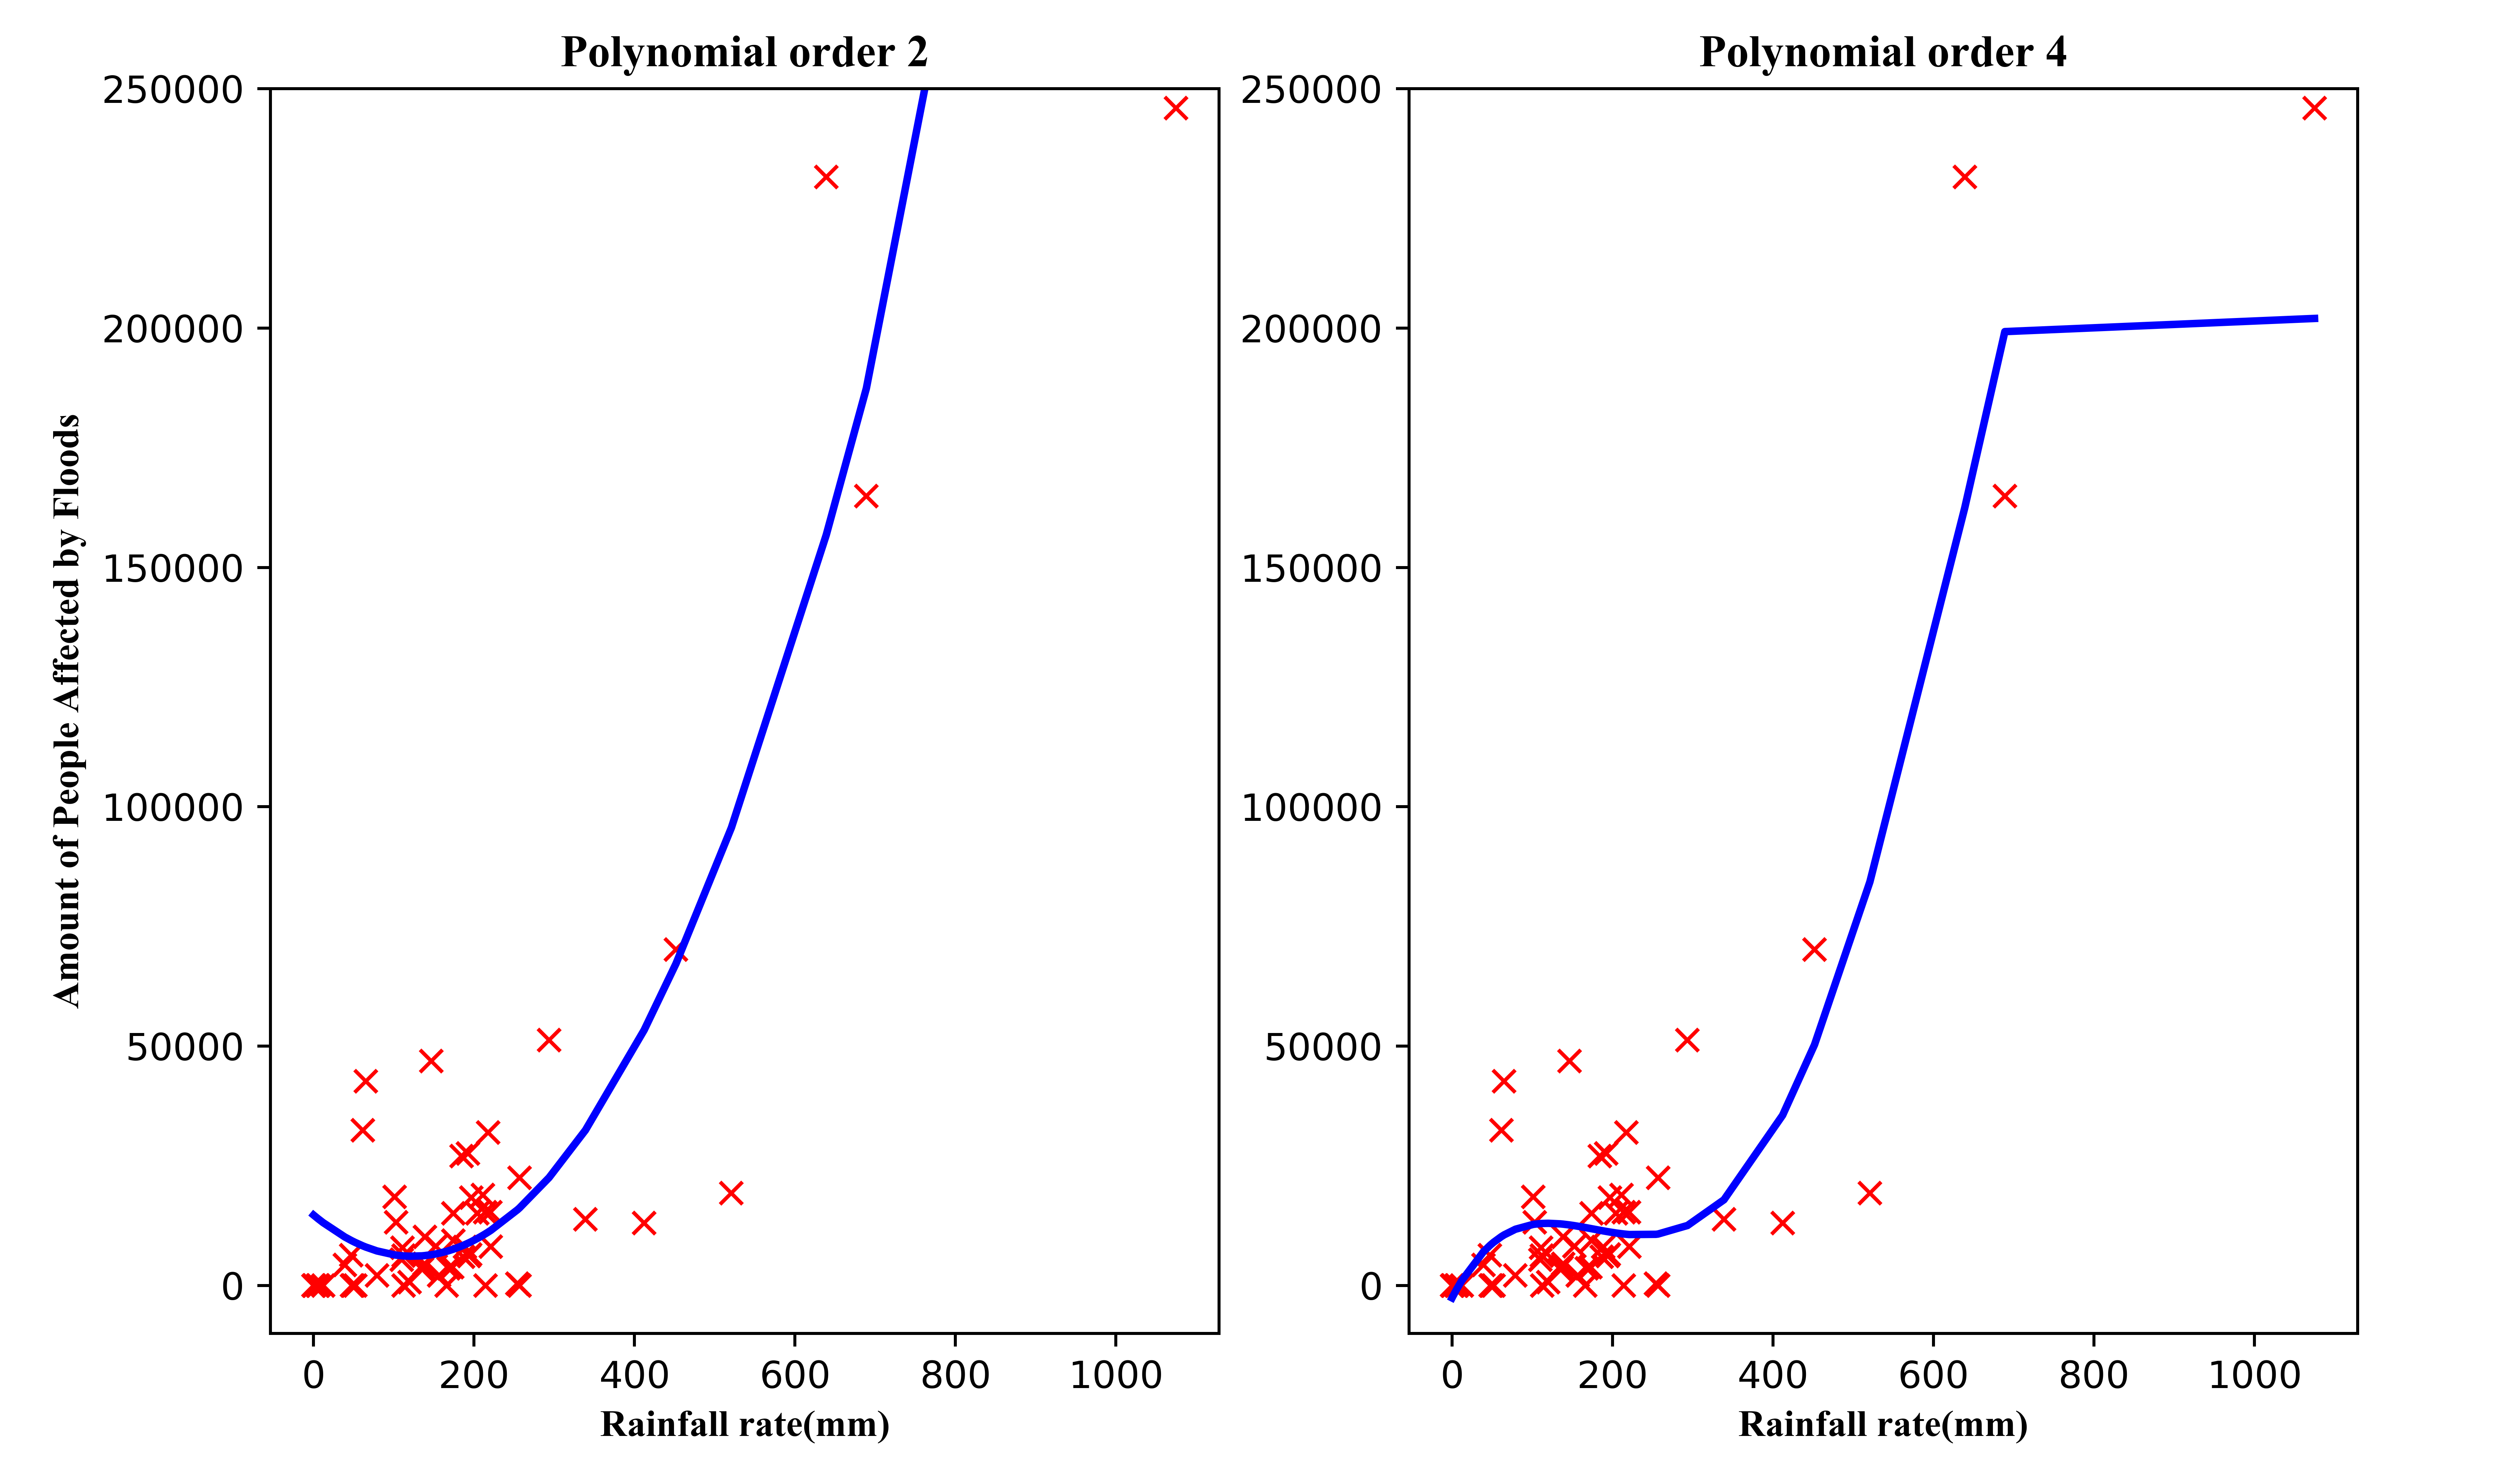
\includegraphics[scale=0.15]{pol24.png}
\caption{Comparison between polynomial regression models with order=2 and order=4}\label{fig=pol24.png}
\end{center}
\end{figure}

\noindent 
In Figure \ref{fig=pol24.png}, it can be concluded that polynomial model with order 2 is slightly underfitting the data points, particularly in the lower region of the graphs. Meanwhile, polynomial model with order 4 is shown some signs of overfitting that won't generalize well with the trends in data points. In Figure \ref{fig=corrrainpeopreg.png}, it can be clearly seen that the polynomial model with order of 3 will yield to the best prediction for this particular problem.\\

\begin{figure}
\begin{center}
\graphicspath{ {./Pict/} }
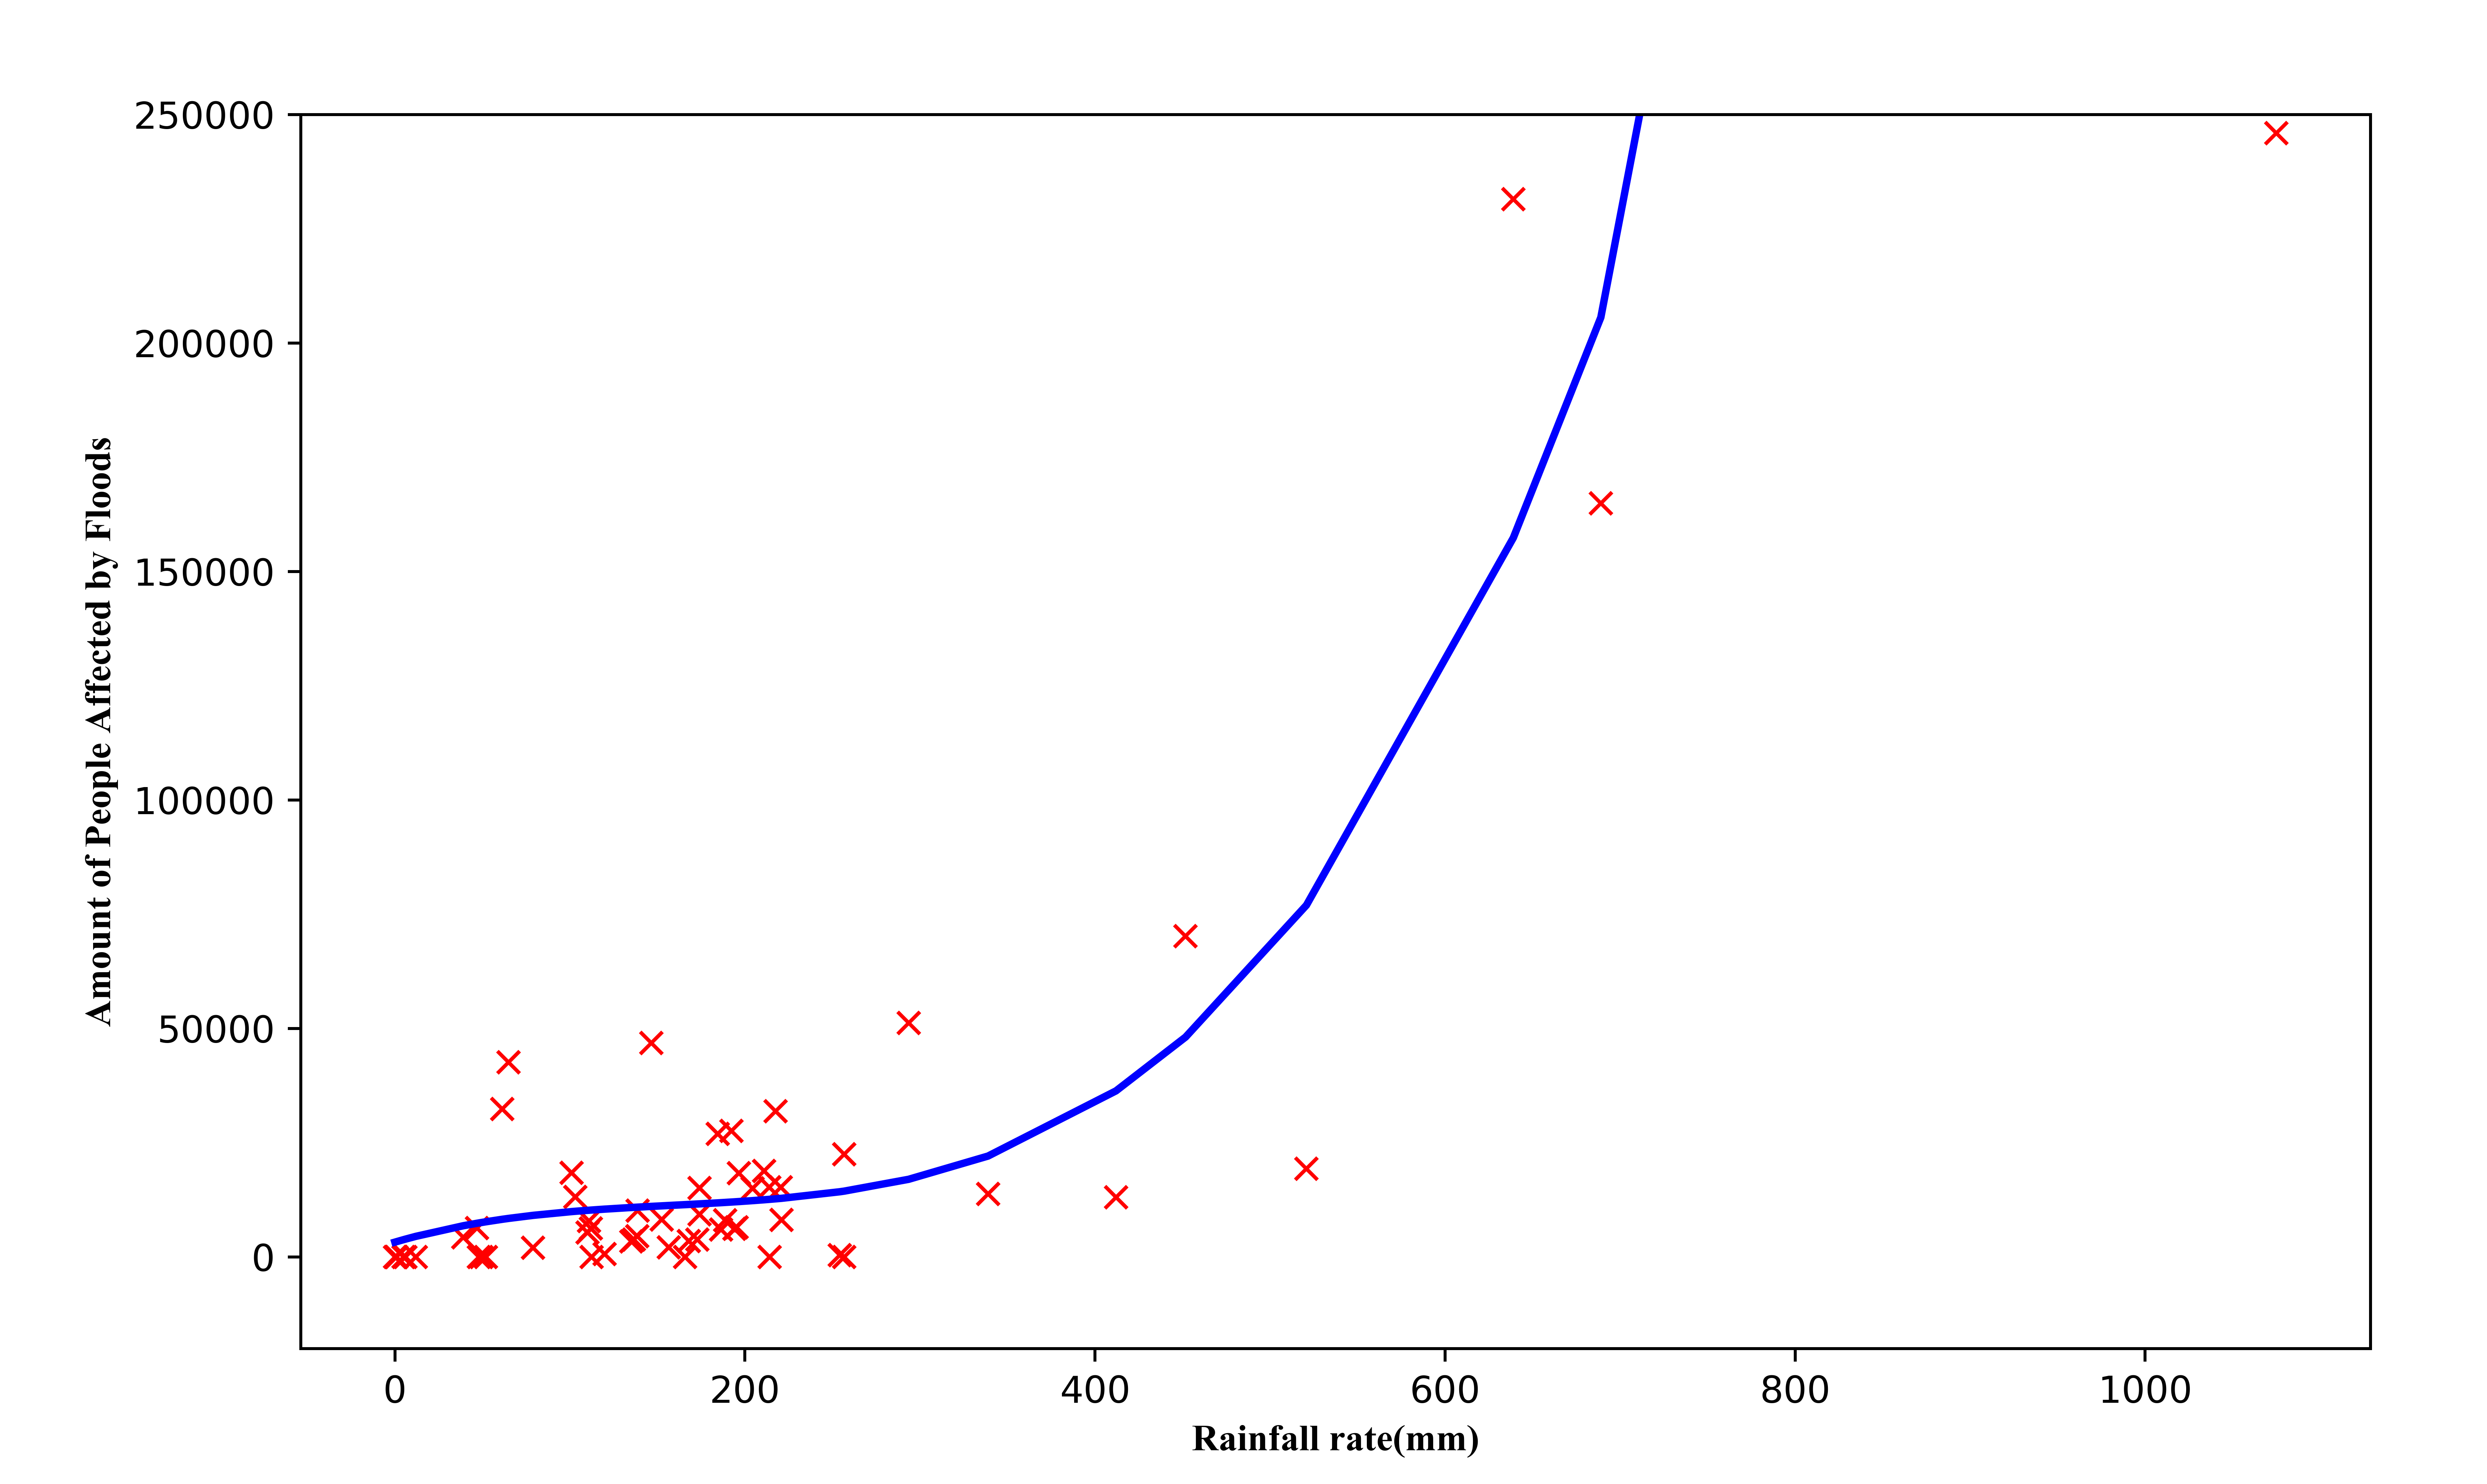
\includegraphics[scale=0.15]{corrrainpeopreg.png}
\caption{Polynomial model with order=3 to estimate the amount of people who will be affected by floods in any given rainfall rate}\label{fig=corrrainpeopreg.png}
\end{center}
\end{figure}
\noindent
With polynomial model with order of 3, now the amount of people who will be affected by floods can be estimated in any given rainfall rate. This would be particularly helpful for the local authorities, the rescue teams, and the medical teams to be prepared once the heavy rainfall pours down the city.



\chapter{Clustering: Finding Out the Districts with High and Low Risks of Floods}

By now, the correlation between rainfall rate and flood occurrences is already known. Moreover, the amount of sub-districts and people that will be affected by floods in any given rainfall rate can be predicted with linear regression model and third order polynomial regression model. Next, the problem is: the authorities now can predict the amount of sub-districts that will be flooded when the heavy rainfall pours down the city, but where should they focus their attention to? is there any particular district that they should take their attention to?\\

\noindent
In order to answer this question, in this chapter, all of the districts in Jakarta will be clustered into certain number of segments. From that, the classification regarding their potential risks of upcoming floods can be concluded.\\

\section{Feature Extractions}
Before clustering all of the districts in Jakarta into several segments, the first that needs to be done is to obtain the list containing the name of all of the districts. This is necessary because the investigation will be conducted at the district level instead of sub-district level to avoid the visualization that is too dense. Afterall, each district also represents several sub-districts. This means that all of the features in each sub-district will be assigned and aggregated to the district in which they are located.\\

\noindent
In order to obtain all of the districts name, web-scraping technique from five different Wikipedia pages is applied. This task can be done with relevant libraries in Python such as pandas and BeautifulSoup to parse the HTML and convert it to a data frame.\\

\noindent
After the extraction of the names of all of the districts in Jakarta, the next step is to obtain the latitude and longitude coordinates of each district. This task can be completed by utilizing geopy library in Python. After all of the necessary information is obtained, then the geospatial visualization of the districts in Jakarta can be shown using folium library. The visualization is shown in Figure \ref{fig=map.png}.\\

\begin{figure}
\begin{center}
\graphicspath{ {./Pict/} }
\includegraphics[scale=0.8]{map.png}
\caption{Geospatial visualization of the districts of Jakarta}\label{fig=map.png}
\end{center}
\end{figure}


\noindent
After visualization, then the features that are relevant for clustering need to be extracted. With meaningful features, then the clustering algorithm such as k-Means would perform better and will give a precise clustering result. In order to obtain meaningful features to help the clustering algorithm to make a clustering decision, more than 30 datasets from Satu Data Indonesia website will be fetched and combined into one data frame.\\

\noindent
Each of the dataset from Satu Data Indonesia contains flood occurrences in Jakarta within a month. The data that are available are the one in the span 2013 until 2016, which means that in total there should be 48 different datasets. However, there were few months where the datasets are unavailable. The missing dataset in certain months wouldn't matter much since for this chapter, the focus is not about predicting the trend, but to segmenting the districts. In order to segment the districts, the most important thing is the aggregation of all of the features to provide meaningful clustering results.\\

\noindent
In the end, the features that are extracted and converted into the final data frame are:
\begin{itemize}
\item The number of cases of floods in each sub-district.
\item The number of people who are affected by floods.
\item The number of people who are forced to relocate from their own house.
\item The number of days needed for each district to recover from each flood occurrence.
\end{itemize}

\section{Determining the Number of Cluster}
For the clustering of the districts in Jakarta, an unsupervised machine learning algorithm, which is k-Means clustering, will be applied. However, before the clustering is conducted, one important thing that should be done in advance is to choose the number of clusters. It is tricky to know the optimum number of cluster in advance without doing a simulation. Applying too little number of cluster would yield to a very high cost function while applying too many number of cluster will yield to meaningless result.\\

\begin{figure}
\begin{center}
\graphicspath{ {./Pict/} }
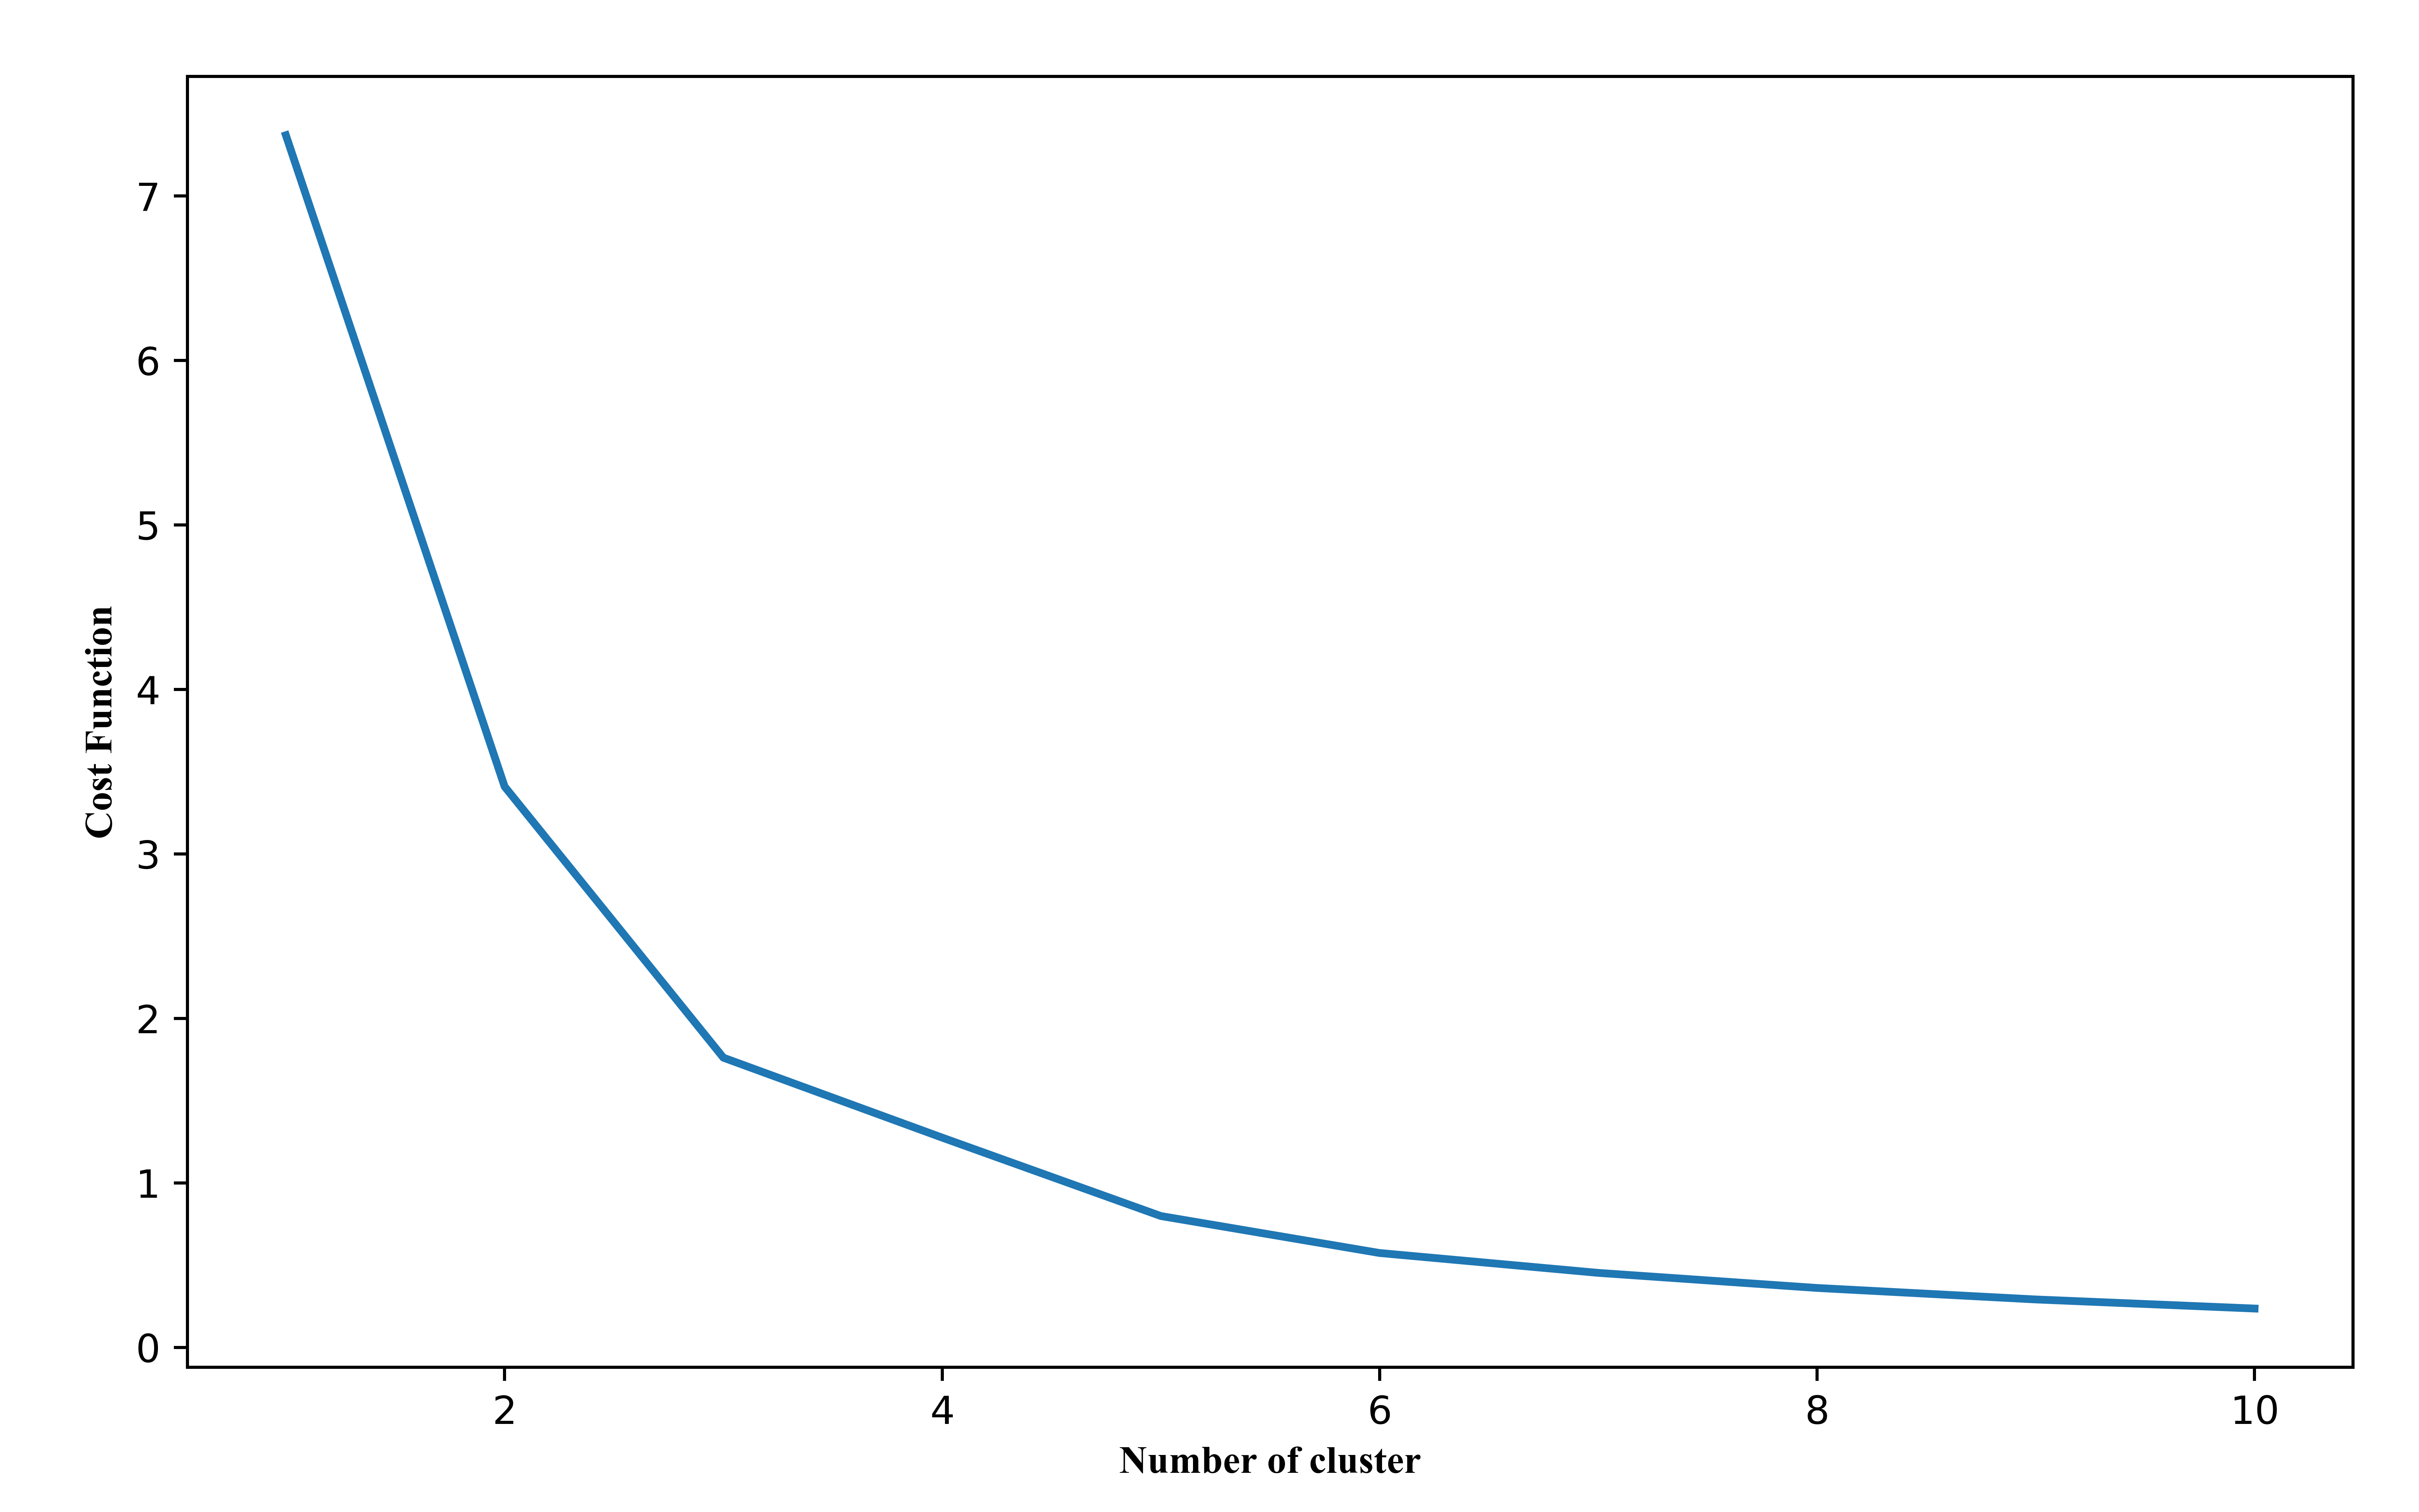
\includegraphics[scale=0.15]{kcluster.png}
\caption{Elbow method to determine optimum number of cluster. Optimum number of cluster= 3}\label{fig=kcluster.png}
\end{center}
\end{figure}

\noindent
In order to know the optimum number of cluster, the elbow method is going to be applied. The elbow method is a very helpful method to get the number of clusters that gives less cost function but at the same time still retains the meaningfulness of the result. Figure \ref{fig=kcluster.png} shows the simulation result of the elbow method. It is clear from the graph that the optimum number of cluster would be 3.

\section{Clustering}
Knowing that 3 clusters will give the optimum result, then the K-Means clustering algorithm can be applied. Figure \ref{fig=cluster.png} shows the clustering result in a map. \\

\begin{figure}
\begin{center}
\graphicspath{ {./Pict/} }
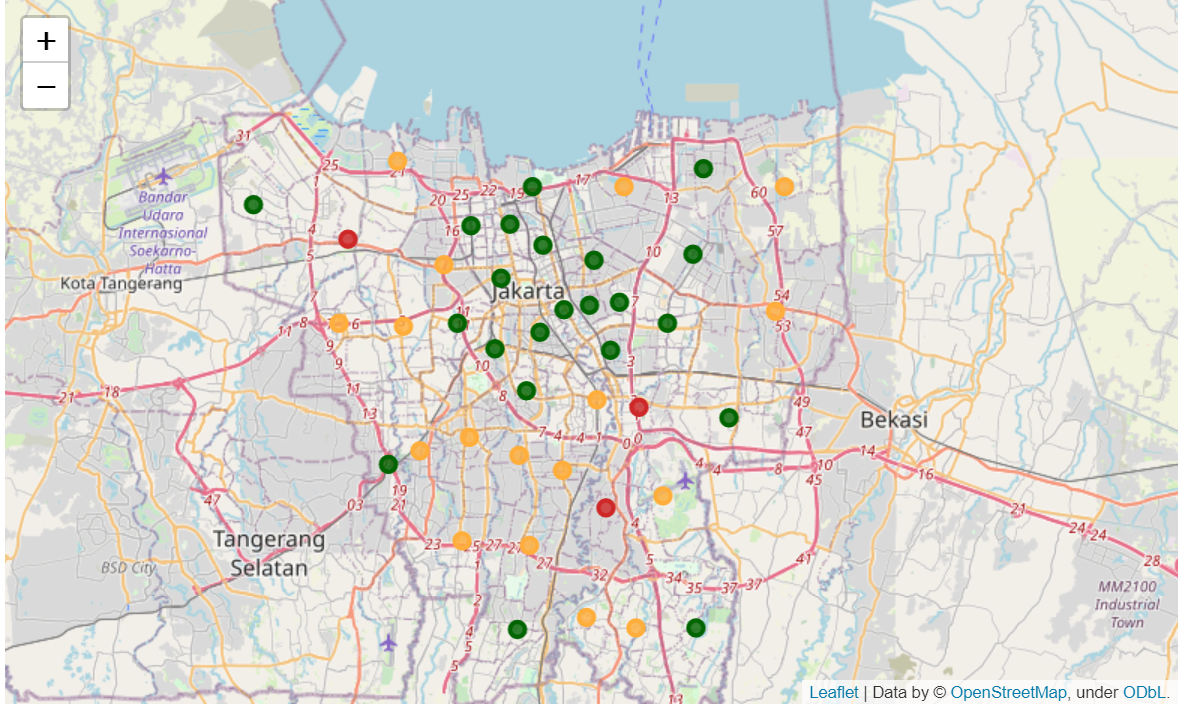
\includegraphics[scale=0.8]{cluster.png}
\caption{Clustering result of the districts of Jakarta. Green: Safe, Orange: Moderate, Red: High Risks of Flooding}\label{fig=cluster.png}
\end{center}
\end{figure}

\noindent
In order to understand better the characteristics of each cluster, Table \ref{tab:1}, Table \ref{tab:2}, and Table \ref{tab:3} give the overview regarding the result for each cluster.\\
\begin{table}
\centering
\caption{Cluster 1: The safest districts in Jakarta}
\label{tab:1}
\begin{adjustbox}{width=\textwidth}
\begin{tabular}{llrrrrrrr}
\toprule
{} &       District &  Latitude &   Longitude &  Cluster Labels &  no. of cases &  no. of People Affected &  no. of People Forced to Relocate &  Days of Flood Recovery \\
\midrule
0  &           Koja & -6.120750 &  106.907362 &               1 &            16 &                  4236.0 &                              6067 &                    52.0 \\
5  &     Pademangan & -6.129052 &  106.828972 &               1 &            12 &                  1935.0 &                              1453 &                    37.0 \\
6  &       Cipayung & -6.329399 &  106.903739 &               1 &            14 &                  1225.0 &                               801 &                    50.0 \\
7  &    Duren Sawit & -6.234138 &  106.919247 &               1 &            10 &                   648.0 &                               150 &                    25.0 \\
8  &      Kalideres & -6.137006 &  106.701594 &               1 &            16 &                 24392.0 &                             14180 &                    66.0 \\
11 &       Palmerah & -6.191002 &  106.794363 &               1 &            10 &                 27987.0 &                             20253 &                    32.0 \\
13 &      Kemayoran & -6.162546 &  106.856890 &               1 &             8 &                   300.0 &                               300 &                    47.0 \\
15 &          Senen & -6.184971 &  106.843235 &               1 &             0 &                     0.0 &                                 0 &                     0.0 \\
18 &     Taman Sari & -6.146142 &  106.818499 &               1 &             6 &                     0.0 &                               659 &                    19.0 \\
21 &       Matraman & -6.203624 &  106.864579 &               1 &             9 &                  2844.0 &                              2259 &                    21.0 \\
22 &         Gambir & -6.170300 &  106.814800 &               1 &             3 &                     0.0 &                                 0 &                     7.0 \\
23 &        Menteng & -6.195026 &  106.832224 &               1 &             2 &                     0.0 &                                 0 &                     6.0 \\
24 &    Pulo Gadung & -6.191109 &  106.890605 &               1 &             0 &                     0.0 &                                 0 &                     0.0 \\
25 &     Johar Baru & -6.183125 &  106.855332 &               1 &             4 &                     0.0 &                                 0 &                    11.0 \\
26 &  Kelapa Gading & -6.159938 &  106.902483 &               1 &            13 &                  6537.0 &                              8667 &                    48.0 \\
28 &      Setiabudi & -6.221706 &  106.826308 &               1 &             4 &                    30.0 &                               690 &                     6.0 \\
30 &        Tambora & -6.146614 &  106.801046 &               1 &            16 &                   523.0 &                             12772 &                    81.0 \\
32 &      Jagakarsa & -6.330101 &  106.822237 &               1 &            17 &                  2736.0 &                              1737 &                    51.0 \\
35 &    Sawah Besar & -6.155891 &  106.833580 &               1 &             9 &                 17376.0 &                               110 &                    17.0 \\
37 &  Cempaka Putih & -6.181214 &  106.868548 &               1 &             1 &                     0.0 &                                 0 &                     2.0 \\
39 &   Pesanggrahan & -6.255458 &  106.763112 &               1 &            22 &                  7589.0 &                              1020 &                    62.0 \\
40 &    Tanah Abang & -6.202400 &  106.811900 &               1 &            14 &                 51860.0 &                             10002 &                    60.0 \\
\bottomrule
\end{tabular}
\end{adjustbox}
\end{table}

\begin{table}
\centering
\caption{Cluster 2: The districts with highest risks of flooding in Jakarta}
\label{tab:2}
\begin{adjustbox}{width=\textwidth}
\begin{tabular}{llrrrrrrr}
\toprule
{} &     District &  Latitude &   Longitude &  Cluster Labels &  no. of cases &  no. of People Affected &  no. of People Forced to Relocate &  Days of Flood Recovery \\
\midrule
12 &  Kramat Jati & -6.274940 &  106.862501 &               2 &            74 &                170580.0 &                             35631 &                   256.0 \\
33 &   Cengkareng & -6.152899 &  106.744718 &               2 &            51 &                828568.0 &                             81643 &                   231.0 \\
36 &   Jatinegara & -6.229147 &  106.877417 &               2 &            64 &                421638.0 &                             52174 &                   312.0 \\
\bottomrule
\end{tabular}
\end{adjustbox}
\end{table}

\begin{table}
\centering
\caption{Cluster 3: The districts with moderate risks of flooding in Jakarta}
\label{tab:3}
\begin{adjustbox}{width=\textwidth}
\begin{tabular}{llrrrrrrr}
\toprule
{} &           District &  Latitude &   Longitude &  Cluster Labels &  no. of cases &  no. of People Affected &  no. of People Forced to Relocate &  Days of Flood Recovery \\
\midrule
1  &           Cilandak & -6.289798 &  106.796926 &               3 &            35 &                 28333.0 &                               913 &                    89.0 \\
2  &          Kembangan & -6.191395 &  106.740586 &               3 &            28 &                 60905.0 &                              1074 &                    72.0 \\
3  &      Tanjung Priok & -6.128858 &  106.870793 &               3 &            28 &                 91260.0 &                             35521 &                    97.0 \\
4  &        Kebon Jeruk & -6.192572 &  106.769725 &               3 &            43 &                177859.0 &                             14695 &                   139.0 \\
9  &             Cakung & -6.185562 &  106.940109 &               3 &            22 &                 25121.0 &                              5614 &                   106.0 \\
10 &            Makasar & -6.269587 &  106.888697 &               3 &            38 &                 33301.0 &                              5101 &                   120.0 \\
14 &        Penjaringan & -6.117265 &  106.767433 &               3 &            28 &                 42330.0 &                             43968 &                   142.0 \\
16 &     Kebayoran Baru & -6.243164 &  106.799850 &               3 &            29 &                 34747.0 &                               524 &                    80.0 \\
17 &       Pasar Minggu & -6.291950 &  106.827835 &               3 &            32 &                 31648.0 &                              7946 &                    93.0 \\
19 &            Ciracas & -6.329635 &  106.876604 &               3 &            26 &                 12941.0 &                               984 &                    60.0 \\
20 &           Pancoran & -6.258085 &  106.842733 &               3 &            43 &                 36566.0 &                             14158 &                   156.0 \\
27 &     Kebayoran Lama & -6.249128 &  106.777782 &               3 &            40 &                 10833.0 &                               801 &                   107.0 \\
29 &              Tebet & -6.226016 &  106.858396 &               3 &            41 &                140138.0 &                             31043 &                   177.0 \\
31 &         Pasar Rebo & -6.324973 &  106.853376 &               3 &            26 &                  4957.0 &                                18 &                    81.0 \\
34 &          Cilincing & -6.129015 &  106.944454 &               3 &            33 &                 45478.0 &                             23646 &                   118.0 \\
38 &  Grogol Petamburan & -6.164188 &  106.788317 &               3 &            31 &                  5746.0 &                              7590 &                   120.0 \\
41 &   Mampang Prapatan & -6.250878 &  106.823021 &               3 &            36 &                  6995.0 &                              2246 &                    81.0 \\
\bottomrule
\end{tabular}
\end{adjustbox}
\end{table}

\noindent
From Table \ref{tab:1} it can be seen that the districts that contained in cluster 1 are the safest districts in Jakarta in terms of their robustness against flooding, although they are not entirely safe. In general, the districts that clustered together in this cluster have the lowest number of flood cases over the span 2013 until 2016 and they also only need short amount of time to recover from floods.\\

\noindent
There are only three districts in cluster 2, as shown in Table \ref{tab:2}. However, these three are the districts with the highest potential to have upcoming floods should a heavy rainfall pours down Jakarta in the future. As shown in the table, these three districts have by far the most cases of floods over the span 2013 until 2016, the most people who are affected by floods, and they also take the longest time to recover from floods. Without a doubt, these three districts are the one that the authorities, the rescue team, and the medical teams should focus their attention the most to.\\

\noindent
In cluster 3, as shown in Table \ref{tab:3}, there are several districts that have lower number in terms of people affected by flood compared to some districts in cluster 1. However, by taking a closer look, all of the districts in cluster 3 have more number of flood cases and they need longer time to recover from floods compared to cluster 1. At the same time, they are also not as severe as the three districts in cluster 2. In conclusion, the districts in cluster 3 are the districts that need moderate amount of attention should a heavy rainfall pours down Jakarta.\\



\chapter{Influence of Parks to Mitigate the Floods}

By now,  the best time to do the preparation to mitigate the severity of floods in Jakarta has been answered. The predictive modeling algorithm to estimate the number of districts as well as civilians that might be affected by floods with given rate of rainfall also have been built. Just now, the authorities are also already know which districts that they should focus their attention to during the heavy rainfall rate periods in Jakarta.\\

\noindent
The only thing that still missing is the question: how should people mitigate the floods? What should they do to mitigate the floods? It is a very tricky question to answer because of the need to use hefty amount of datasets with different variety of topics to find the solution.\\
 
\noindent
Unfortunately, there is no open dataset that might be helpful to answer this question. Also, the scope will be even broader if socioeconomics or sociological situation like the growing rate of populations or people's behavior on how they maintain the cleanliness of their environments are considered. The correlation between socieconomics or sociological situation with the occurrence of floods will be out of the scope of this project.\\

\noindent
Thus, to try to answer this question, a rather simplistic approach will be conducted. With Foursquare API, the parks nearby each district will be fetched. Then, the possible correlation between the amount of parks and the severity of floods will be investigated.\\

\noindent
In order to make sure that only venues with parks category will be returned, it is necessary to define the category ID of parks in advance before calling the API. Detailed information about different ID categories depending on the type of venues can be found in the Foursquare Developers page. Table \ref{tab:4} shows the output after Foursquare API was called.\\

\begin{table}
\centering
\caption{First five rows of places with parks category that were returned by Foursquare API}
\label{tab:4}
\begin{adjustbox}{width=\textwidth}
\begin{tabular}{llrrlrr}
\toprule
{} & District &  Latitude &   Longitude &                        Venue &  Venue Latitude &  Venue Longitude \\
\midrule
0 &     Koja &  -6.12075 &  106.907362 &            Taman Walang Baru &       -6.120104 &       106.905190 \\
1 &     Koja &  -6.12075 &  106.907362 &  JL. Lagoa Terusan gg. II C2 &       -6.110252 &       106.910098 \\
2 &     Koja &  -6.12075 &  106.907362 &                 Tanjungpriok &       -6.113818 &       106.893159 \\
3 &     Koja &  -6.12075 &  106.907362 &              Mochie's castle &       -6.131510 &       106.921496 \\
4 &     Koja &  -6.12075 &  106.907362 &  Food Park Mall Of Indonesia &       -6.118548 &       106.900294 \\
\bottomrule
\end{tabular}
\end{adjustbox}
\end{table}

\noindent
The first data that were returned from Foursquare API didn't look very good although the desired category of the place have already been defined in advance. The data contains not only parks, but also some other non-relevant places like restaurant and other places.  In order to fix this and to make sure that at the end the real parks is obtained, then the data needs to be filtered. All of the venues which doesn't contain the word 'taman', which is the Indonesian word for parks, will be excluded from the data. Table \ref{tab:5} shows the filtered data.\\

\begin{table}
\centering
\caption{Filtered table which only contains the real parks}
\label{tab:5}
\begin{adjustbox}{width=\textwidth}
\begin{tabular}{lrlrrlrr}
\toprule
{} &  index &   District &  Latitude &   Longitude &                Venue &  Venue Latitude &  Venue Longitude \\
\midrule
0 &      0 &       Koja & -6.120750 &  106.907362 &    Taman Walang Baru &       -6.120104 &       106.905190 \\
1 &      5 &   Cilandak & -6.289798 &  106.796926 &          Taman Gajah &       -6.277217 &       106.799566 \\
2 &     10 &   Cilandak & -6.289798 &  106.796926 &  Taman Tridarma Raya &       -6.303318 &       106.805154 \\
3 &     13 &  Kembangan & -6.191395 &  106.740586 &    Taman Meruya Ilir &       -6.195407 &       106.740664 \\
4 &     15 &  Kembangan & -6.191395 &  106.740586 &         Taman blok H &       -6.194011 &       106.737629 \\
\bottomrule
\end{tabular}
\end{adjustbox}
\end{table}

\noindent
From the filtered data, then the distribution of the amount of parks in Jakarta can be visualized using histogram. Figure \ref{fig=hist.png} shows the distribution of the amount of parks in Jakarta.\\


\begin{figure}
\begin{center}
\graphicspath{ {./Pict/} }
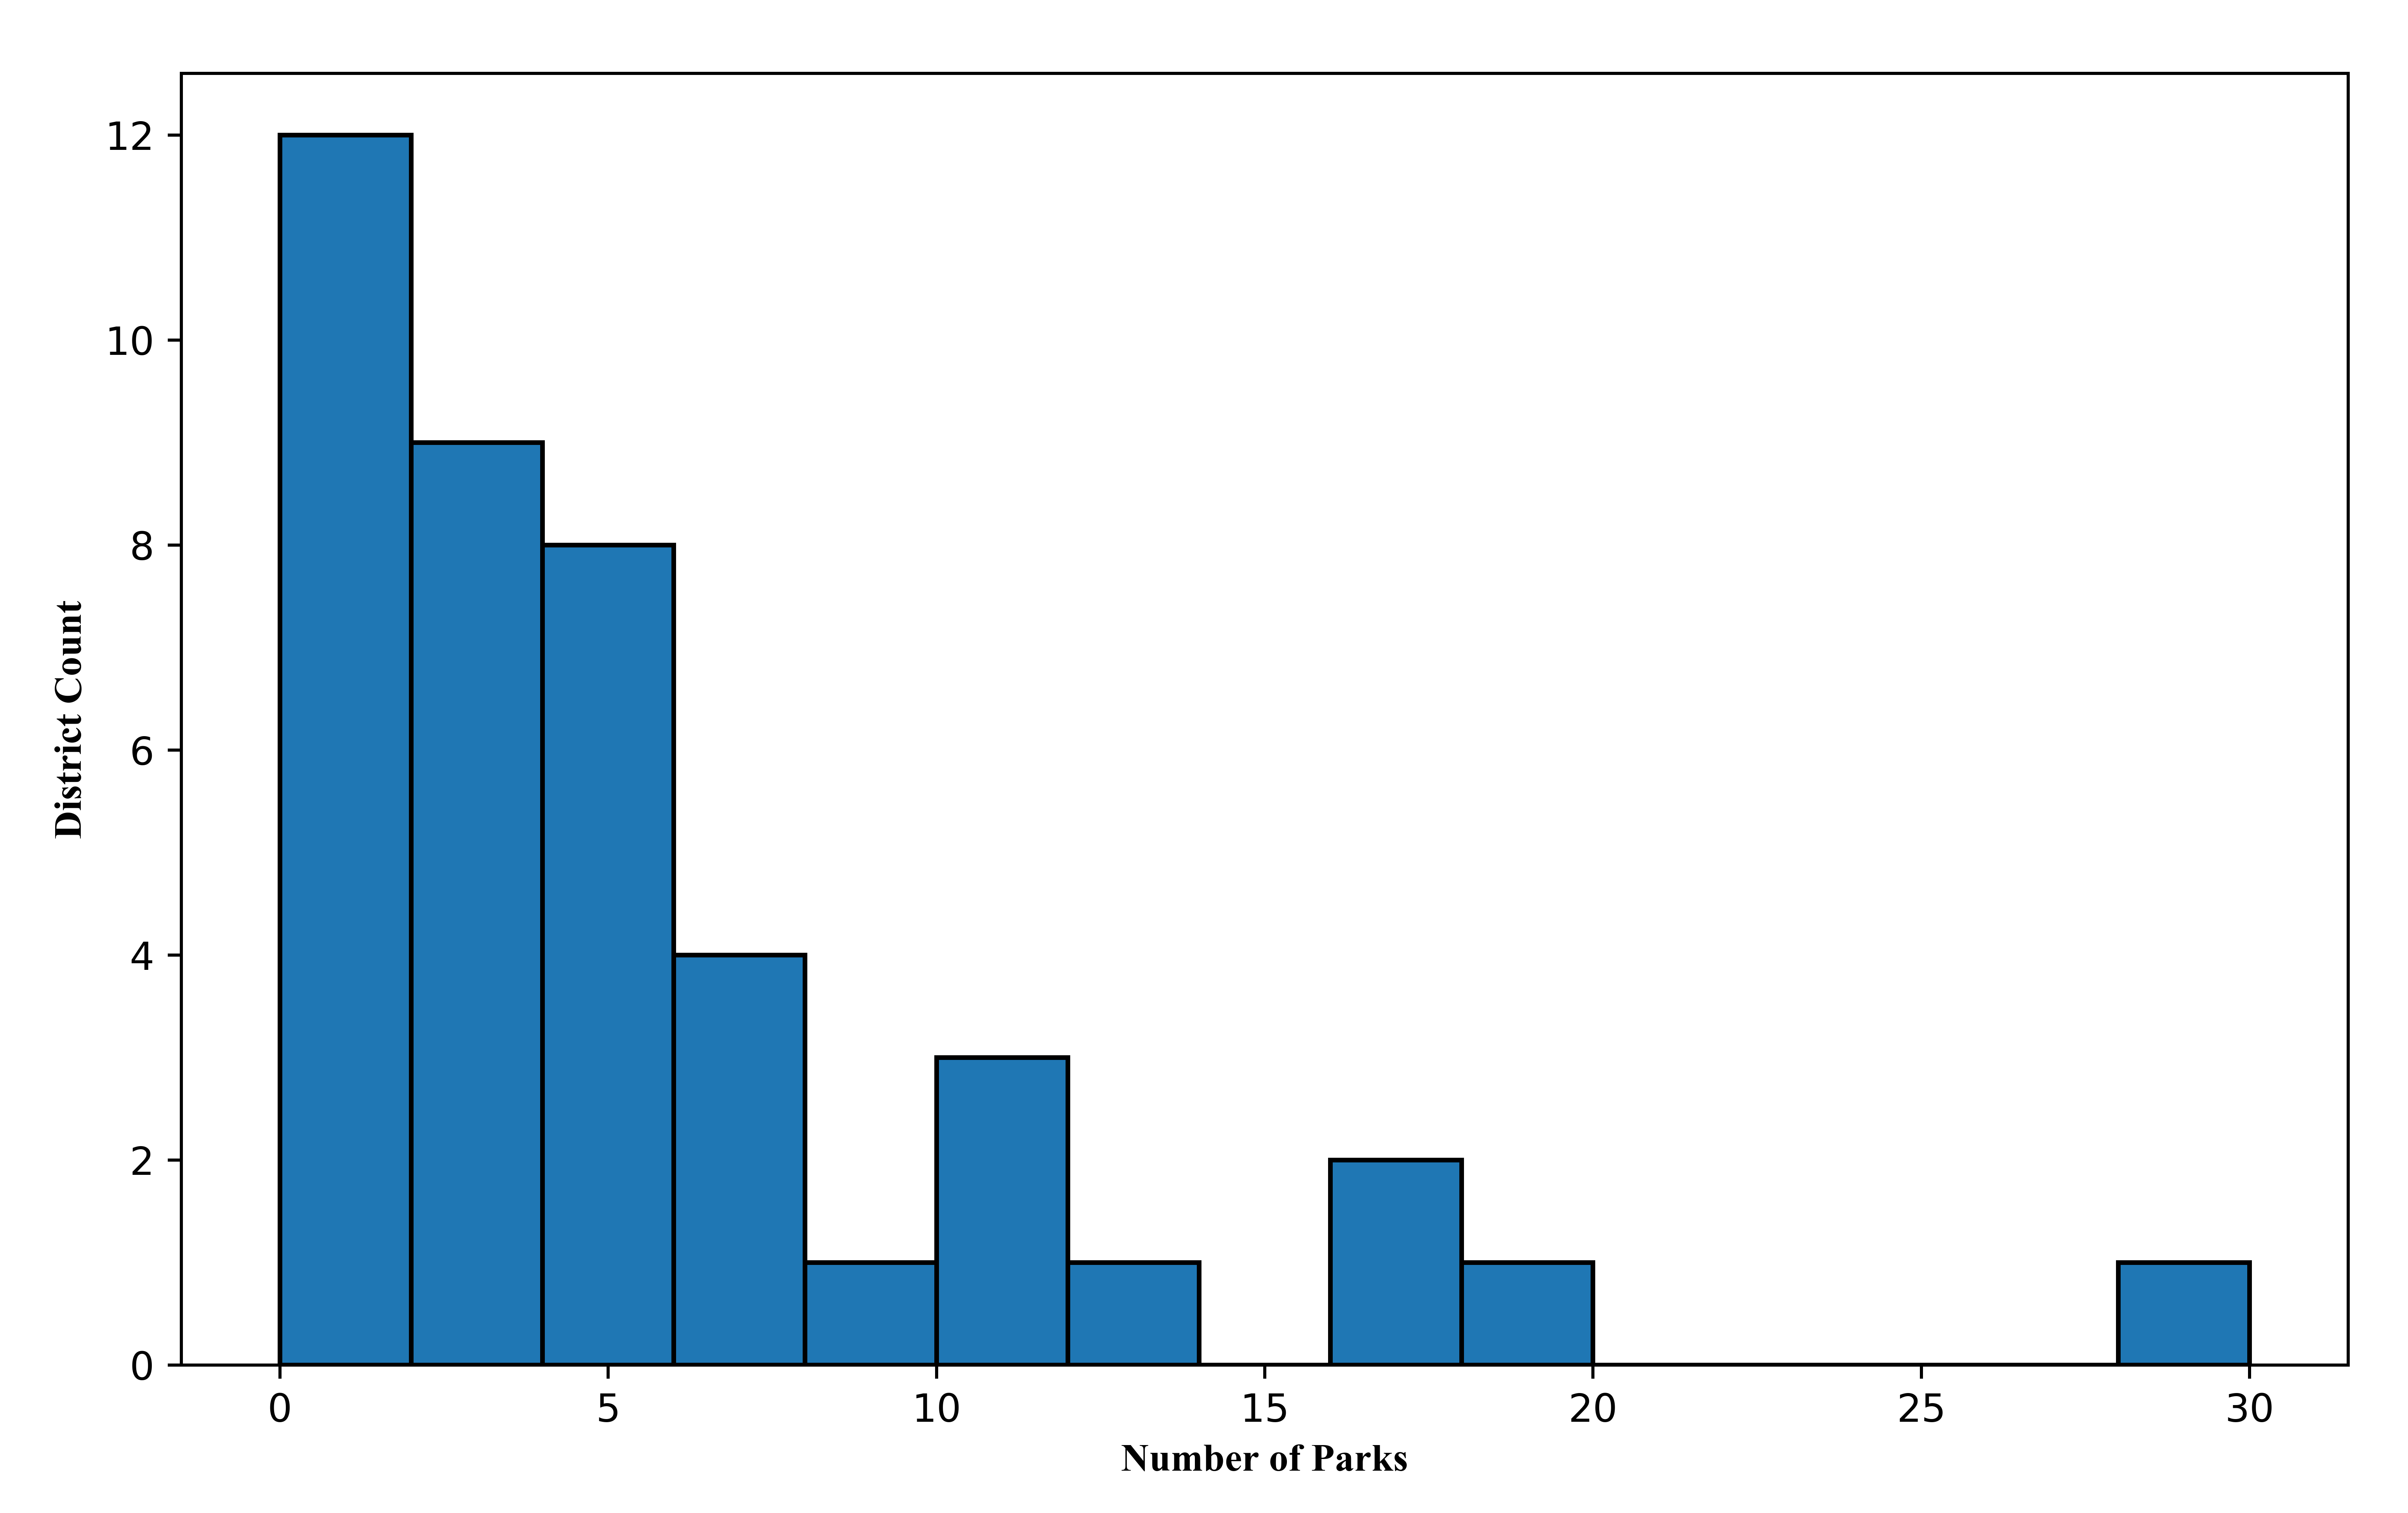
\includegraphics[scale=0.15]{hist.png}
\caption{Distributions of parks among Jakarta districts}\label{fig=hist.png}
\end{center}
\end{figure}

\noindent
As clearly seen from the histogram in Figure \ref{fig=hist.png}, the distribution of the amount of parks in Jakarta is heavily right-skewed. This means that the majority of the districts in Jakarta have a small number of parks. In fact, only 8 out of 41 districts have 10 or more parks. This is also one the problem in Jakarta that it is so congested with residential building and skyscrapers that there are not too many green spaces in the city.\\ 

\noindent
Having the data regarding the amount of parks in each district and then joined this data with the original data frame, then the correlation between them can be investigated. For this purpose, Pearson's correlation method is used. The Table \ref{tab:6} shows the Person's correlation results of all of the features in the data frame.\\

\begin{table}
\centering
\caption{Pearson's correlation result between features in the data frame}
\label{tab:6}
\begin{adjustbox}{width=\textwidth}
\begin{tabular}{lrrrrr}
\toprule
{} &  no. of cases &  no. of People Affected &  no. of People Forced to Relocate &  Days of Flood Recovery &      Park \\
\midrule
no. of cases                     &      1.000000 &                0.574098 &                          0.622585 &                0.942140 & -0.246997 \\
no. of People Affected           &      0.574098 &                1.000000 &                          0.854797 &                0.693484 & -0.188454 \\
no. of People Forced to Relocate &      0.622585 &                0.854797 &                          1.000000 &                0.780099 & -0.255296 \\
Days of Flood Recovery           &      0.942140 &                0.693484 &                          0.780099 &                1.000000 & -0.281488 \\
Park                             &     -0.246997 &               -0.188454 &                         -0.255296 &               -0.281488 &  1.000000 \\
\bottomrule
\end{tabular}
\end{adjustbox}
\end{table}

\noindent
From Table \ref{tab:6}, it can be concluded that the amount of parks in each district doesn't have a significant association with the severity of the floods. The Pearson's correlations between the amount of parks with different set of features are all in around -0.2. However, this negative correlation does makes sense since the more a district has a park, then the less the severity of the floods would be. It is important to note that the causality relationship between the amount of parks and the severity of floods cannot be drawn because no random assignment is involved.\\

\noindent
Nonetheless, although the amount of parks doesn't have a significant correlation with the severity of floods, but it is enough to encourage the districts to open up more green spaces in their area. Finally, Figure \ref{fig=parks.png} shows the data points between the amount of parks and the days needed for the districts to recover from flood.\\

\begin{figure}
\begin{center}
\graphicspath{ {./Pict/} }
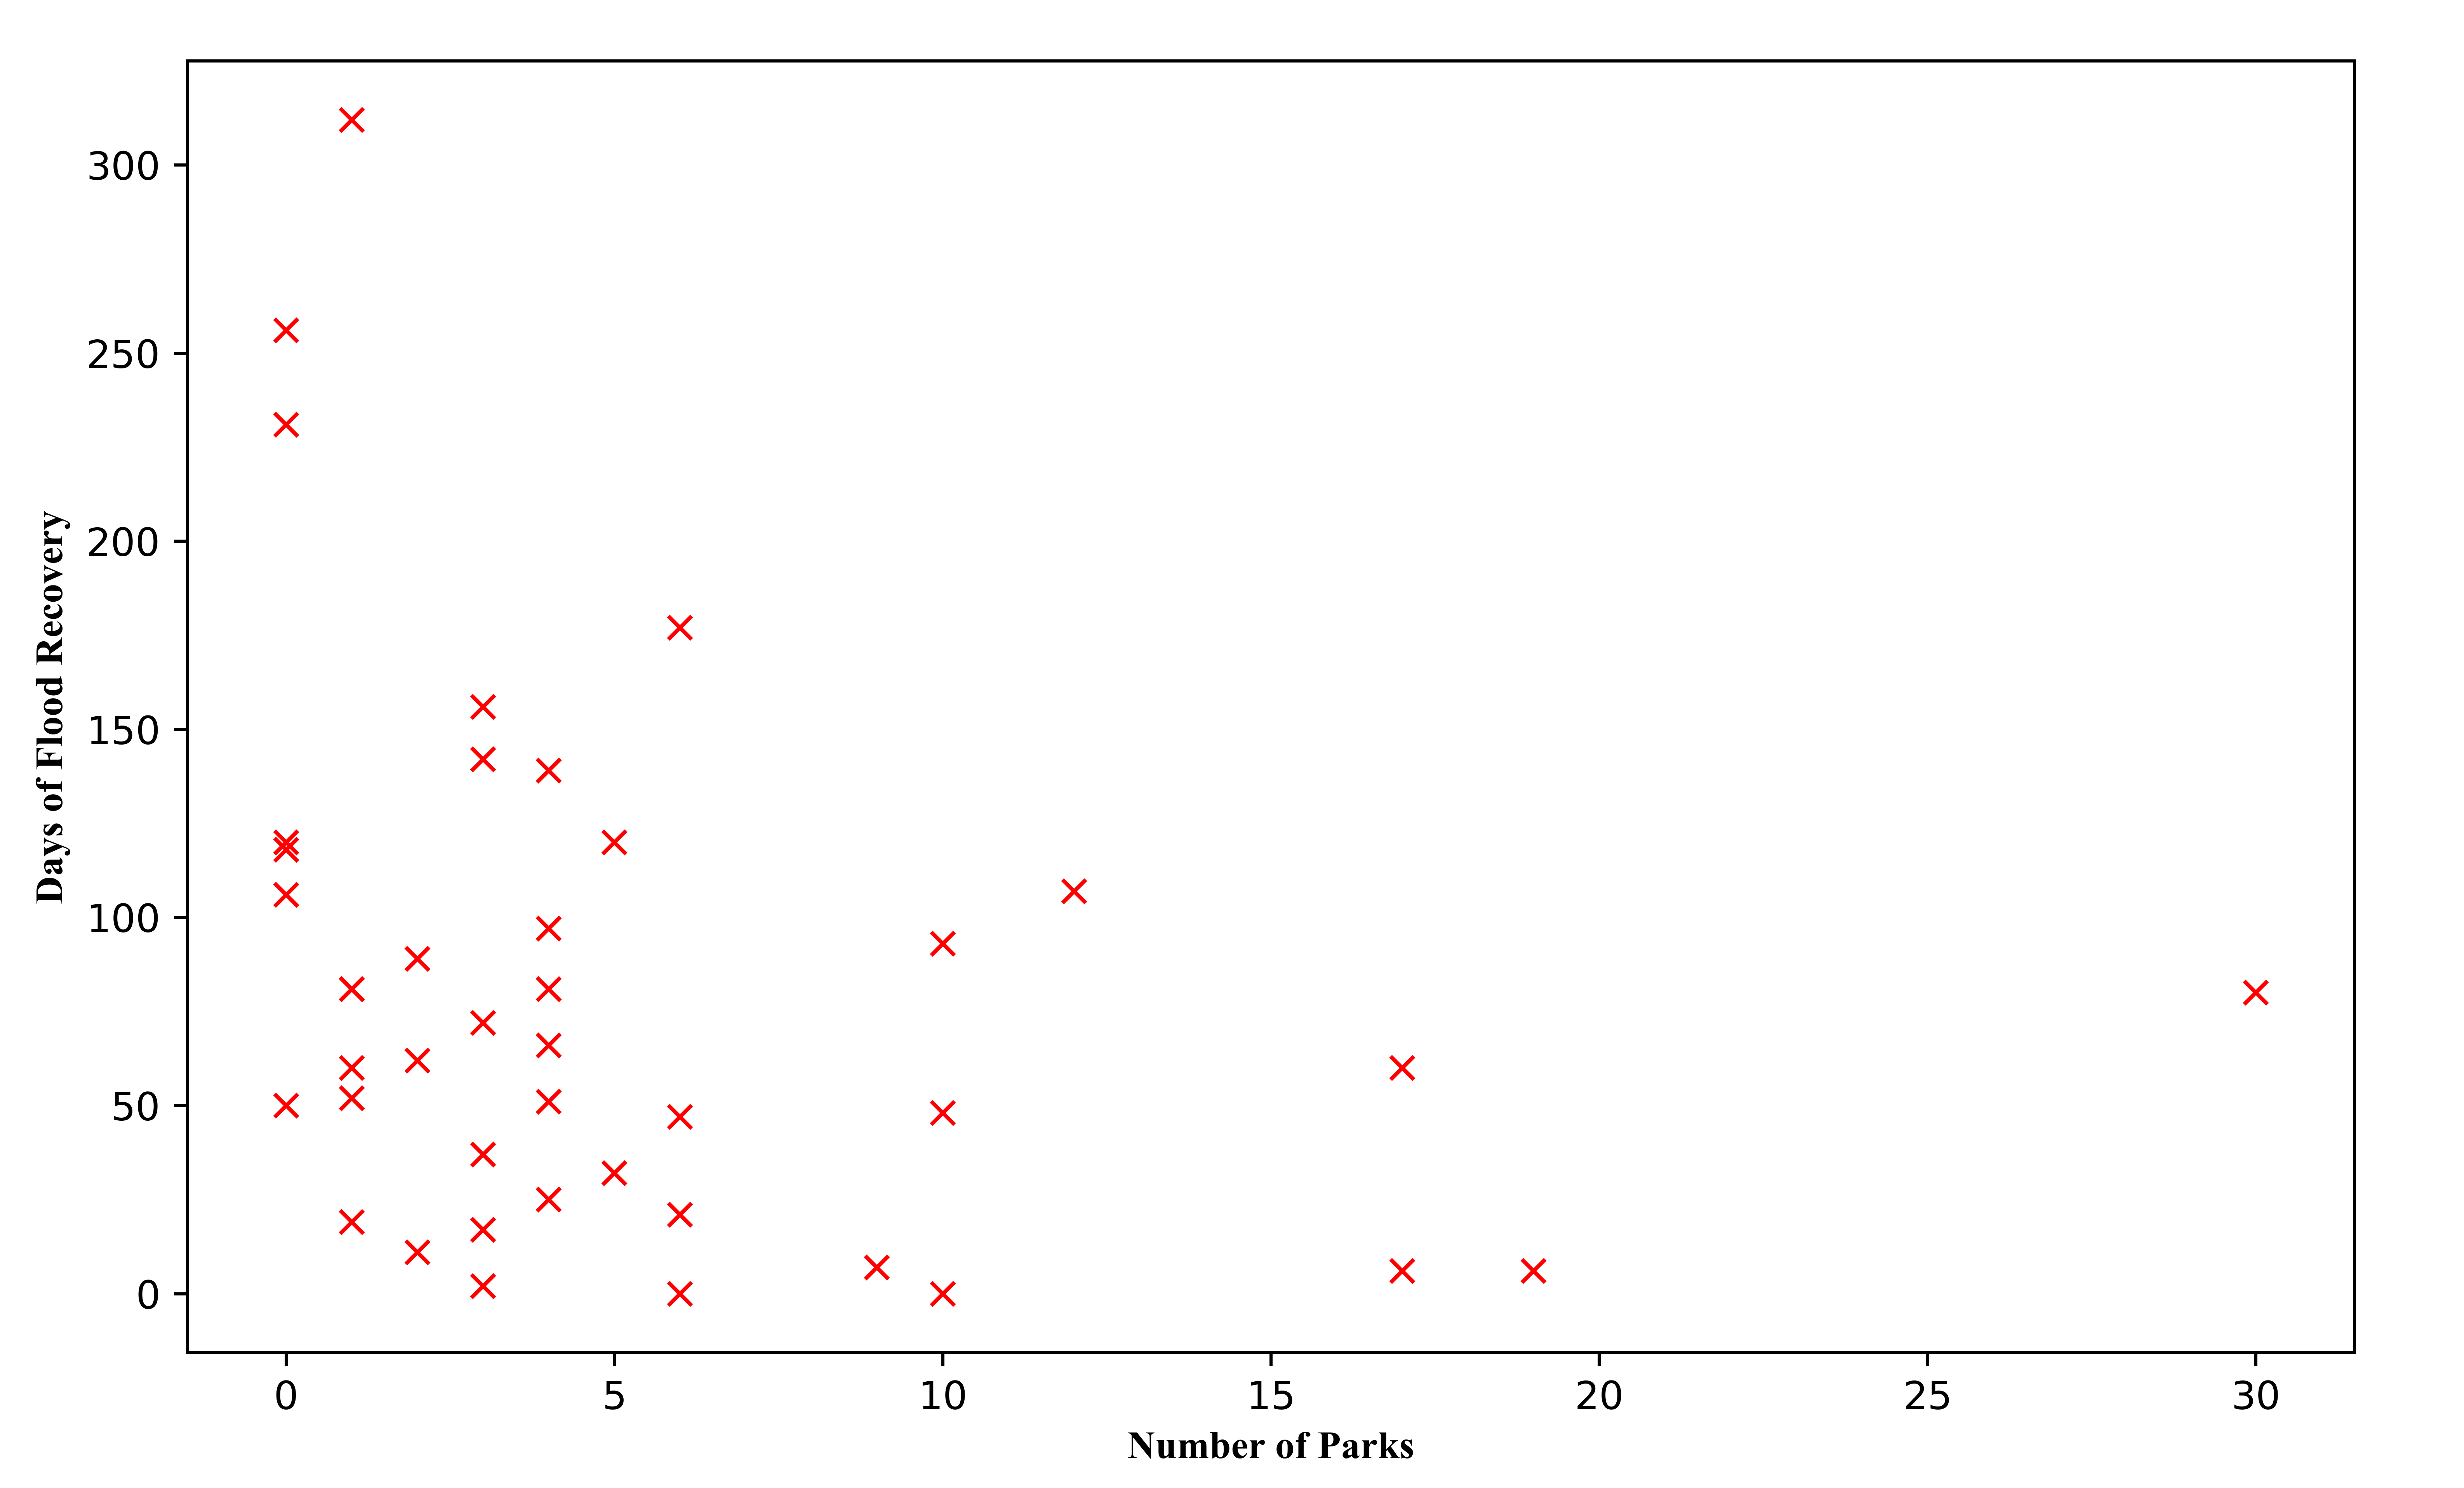
\includegraphics[scale=0.15]{parks.png}
\caption{Data points between the number of parks and the days needed for districts to recover from flood}\label{fig=parks.png}
\end{center}
\end{figure}

\chapter{Summary and Conclusion}

As stated already in the introduction, the main goal of this project is to understand more the nature of Jakarta floods by utilizing the data. There are in total four different chapters in this project:\\ 

\noindent
\textbf{In the first chapter}, the association between rainfall rate and flood occurrences in Jakarta's sub-districts is investigated. With the possible correlation between two variables, the suggestion regarding the best period of time in a year for the authorities to do precautionary and mitigation measurements is given.\\

\noindent
\textbf{In the second chapter}, two predictive modeling algorithm with regression model are built in order to predict or estimate the number of sub-districts and people that will be affected by floods with any given rainfall rate. The number of sub-districts that will be affected by floods can be estimated with linear regression model, while the amount of people who will be affected by floods can be estimated with third order polynomial regression model.\\

\noindent
\textbf{In the third chapter}, the districts in Jakarta is clustered into three segments in order to classify them based on how high their potential risks and severity should a heavy rainfall pours down Jakarta. With the clustering, it clears all of the doubts about which districts that the authorities should focus their attention to during heavy rainfall.\\ 

\noindent
\textbf{In the fourth chapter}, one possible solution to mitigate the floods, which is the amount of parks in any given districts, is discussed. The finding showed that there is no significant correlation between the amount of parks and the severity of floods. However, the amount of parks and severity of floods have a negative correlation, which means that having more parks indeed would be helpful to slightly reduce the severity of floods in any given district.

\begin{thebibliography}{1}
	\bibitem{Wikipedia}
		Daftar kecamatan dan kelurahan di Kota Administrasi Jakarta Pusat, 
		\url{https://id.wikipedia.org/wiki/Daftar_kecamatan_dan_kelurahan_di_Kota_Administrasi_Jakarta_Pusat}
	\bibitem{Wikipedia2}
		Daftar kecamatan dan kelurahan di Kota Administrasi Jakarta Utara, 
		\url{https://id.wikipedia.org/wiki/Daftar_kecamatan_dan_kelurahan_di_Kota_Administrasi_Jakarta_Utara}
	\bibitem{Wikipedia3}
		Daftar kecamatan dan kelurahan di Kota Administrasi Jakarta Timur, 
		\url{https://id.wikipedia.org/wiki/Daftar_kecamatan_dan_kelurahan_di_Kota_Administrasi_Jakarta_Timur}
	\bibitem{Wikipedia4}
		Daftar kecamatan dan kelurahan di Kota Administrasi Jakarta Selatan, 
		\url{https://id.wikipedia.org/wiki/Daftar_kecamatan_dan_kelurahan_di_Kota_Administrasi_Jakarta_Selatan}
	\bibitem{Wikipedia5}
		Daftar kecamatan dan kelurahan di Kota Administrasi Jakarta Barat, 
		\url{https://id.wikipedia.org/wiki/Daftar_kecamatan_dan_kelurahan_di_Kota_Administrasi_Jakarta_Barat}
	\bibitem{SDI}
		Satu Data Indonesia, 
		\url{https://data.go.id}
	\bibitem{BPS}
		Badan Pusat Statistik, 
		\url{https://www.bps.go.id/}
	\bibitem{FAPI}
		Foursquare Developers, \url{https://developer.foursquare.com/docs/build-with-foursquare/categories/}
	
\end{thebibliography}

\addcontentsline{toc}{chapter}{Bibliography}

\end{document}